\documentclass[final]{cpecmu}

%% This is a sample document demonstrating how to use the CPECMU
%% project template. If you are having trouble, see "cpecmu.pdf" for
%% documentation.

\projectNo{P809-2}
\acadyear{2023}

\titleTH{แพลตฟอร์มการแลกเปลี่ยนความคิดสร้างสรรค์ดิจิทัล: การเสริมสร้างการเรียนรู้ผ่าน Gallery Walk}
\titleEN{Digital Creativity Exchange Platform: Enhancing Learning through Gallery Walk}

\author{นายญาณาธิป ภู่สว่าง}{Yanatip Bhoosawang}{630612097}
\author{นางสาวณัฐวรรณ เรียบเรียง}{Nuttawan Reabreang}{630612099}
\author{นายปัณฑ์ธร กันทรัพย์}{Panthon Kansap}{630612105}

\cpeadvisor{dome}
\cpecommittee{chinawat}
\cpecommittee{thanatip}
% \committee{รศ.ดร.\,นิพนธ์ ธีรอำพน}{Assoc.\,Prof.\,Nipon Theera-Umpon, Ph.D.}

%% Some possible packages to include:
\usepackage[final]{graphicx} % for including graphics
\usepackage{cite}

%% Add bookmarks and hyperlinks in the document.
\PassOptionsToPackage{hyphens}{url}
\usepackage[colorlinks=true,allcolors=Blue4,citecolor=red,linktoc=all]{hyperref}
\def\UrlLeft#1\UrlRight{$#1$}

%% Needed just by this example, but maybe not by most reports
\usepackage{afterpage} % for outputting
\usepackage{pdflscape} % for landscape figures and tables. 

%% Some other useful packages. Look these up to find out how to use
%% them.
% \usepackage{natbib}    % for author-year citation styles
% \usepackage{txfonts}
% \usepackage{appendix}  % for appendices on a per-chapter basis
% \usepackage{xtab}      % for tables that go over multiple pages
% \usepackage{subfigure} % for subfigures within a figure
% \usepackage{pstricks,pdftricks} % for access to special PostScript and PDF commands
% \usepackage{nomencl}   % if you have a list of abbreviations

%% if you're having problems with overfull boxes, you may need to increase
%% the tolerance to 9999
% \tolerance=9999

% \bibliographystyle{plain}
% \bibliographystyle{IEEEbib}
\bibliographystyle{IEEEtran}


% \renewcommand{\topfraction}{0.85}
% \renewcommand{\textfraction}{0.1}
% \renewcommand{\floatpagefraction}{0.75}

%% Example for glossary entry
%% Need to use glossary option
%% See glossaries package for complete documentation.
\ifglossary
  \newglossaryentry{lorem ipsum}{
    name=lorem ipsum,
    description={derived from Latin dolorem ipsum, translated as ``pain itself''}
  }
\fi

%% Uncomment this command to preview only specified LaTeX file(s)
%% imported with \include command below.
%% Any other file imported via \include but not specified here will not
%% be previewed.
%% Useful if your report is large, as you might not want to build
%% the entire file when editing a certain part of your report.
% \includeonly{chapters/intro,chapters/background}

\begin{document}
\maketitle
\makesignature

\ifproject
\begin{abstractTH}

ในปัจจุบันปัญหาด้านสุขภาพของประชากรมีแนวโน้มจะสูงขึ้นเรื่อย ๆ ประกอบกับการเข้าสู่สังคมสูงวัยของประชากร ปัญหาสุขภาพจึงเป็นปัญหาที่สำคัญ ซึ่งส่งผลกระทบต่อชีวิตของประชากรโดยส่วนมาก มะเร็งช่องปากเป็นมะเร็งชนิดหนึ่งที่พบมากในกลุ่มประชากรที่มีอายุตั้งแต่ 40 ปีขึ้นไป ที่มีประวัติด้านการสูบบุหรี่ และ
/หรือดื่มแอลกอฮอล์ และเคี้ยวหมาก ซึ่งการตรวจสอบรอยโรคในระยะแรกอาจทำได้ยากโดยทั่วไปและหากปล่อยเป็นระยะเวลานานเกินไปอาจทำให้รอยโรคลุกลามเป็นมะเร็งได้ในที่สุด คณะผู้จัดทำมีความสนใจ
ในเรื่องนี้ จึงได้จัดทำดิจิทัลแพลตฟอร์มเพื่อรองรับระบบปัญญาประดิษฐ์ (AI) เพื่อใช้ในการตรวจสอบและคัดกรองรอยโรคก่อนมะเร็งช่องปากและมะเร็งช่องปาก ที่ใช้ร่วมกับการประเมินจากทันตแพทย์ผู้เชี่ยวชาญ

คณะผู้จัดทำจึงได้นำเสนอการพัฒนาเว็บแอปพลิเคชัน ซึ่งเป็นแพลตฟอร์มดิจิทัลสำหรับรองรับระบบปัญ-ญาประดิษฐ์ (AI) เพื่อตรวจคัดกรองและเฝ้าระวังการเกิดรอยโรคก่อนมะเร็งและมะเร็งช่องปาก (Digital Platform for Detecting and Analyzing Oral Potentially Malignant Disorders and Oral Cancer) โดยกลุ่มผู้ใช้งานของดิจิทัลแพลตฟอร์มนี้จะเป็นทันตแพทย์ทั่วประเทศและประชากรทั่วไปที่มีความสน ใจในการนำดิจิทัลแพลตฟอร์มนี้ไปใช้

คณะผู้จัดทำหวังว่า ดิจิทัลแพลตฟอร์มนี้จะส่งผลให้ทันตแพทย์ทั่วประเทศสามารถตรวจหามะเร็งช่องปากได้อย่างรวดเร็ว และเป็นเครื่องมือหนึ่งที่จะช่วยแก้ไขปัญหาด้านสุขภาพของประชากรโดยเฉพาะมะเร็งช่องปากได้อย่างมีประสิทธิภาพ
\end{abstractTH}

\begin{abstract}

At present, the health problems of the population tend to increase more and more, together with the population entering an aging society. Health problems are therefore important. which affects the lives of the majority of the population Oral cancer is a type of cancer that is most commonly found in people aged 40 and over who have a history of smoking and/or drink alcohol and chew betel nuts. Detecting the Oral Cancer in its early stages may be difficult in general, and if left for too long, it may eventually cause the lesion to develop into cancer. The organizing team is interested.
In this regard, a digital platform has been created to support artificial intelligence (AI) systems for use in examining and screening Oral Potentially Malignant Disorders and Oral Cancer. used in conjunction with an evaluation from an expert dentist.

The team therefore presented the development of a web application. which is a digital platform for supporting the artificial intelligence (AI) system for Detecting and Analyzing Oral Potentially Malignant Disorders and Oral Cancer by a group of The users of this digital platform will be dentists across the country and the general population who are interested in using this digital platform.

The organizing team hopes that this digital platform will allow dentists across the country to quickly detect oral cancer. And it is one tool that will help effectively solve the health problems of the population, especially oral cancer.
\end{abstract}

\iffalse
\begin{dedication}
This document is dedicated to all Chiang Mai University students.

Dedication page is optional.
\end{dedication}
\fi % \iffalse

\begin{acknowledgments}
Your acknowledgments go here. Make sure it sits inside the
\texttt{acknowledgment} environment.

\acksign{2020}{5}{25}
\end{acknowledgments}%
\fi % \ifproject

\contentspage

\ifproject
\figurelistpage

\tablelistpage
\fi % \ifproject

% \abbrlist % this page is optional

% \symlist % this page is optional

% \preface % this section is optional


\pagestyle{empty}\cleardoublepage
\normalspacing \setcounter{page}{1} \pagenumbering{arabic} \pagestyle{cpecmu}

\chapter{\ifenglish Introduction\else บทนำ\fi}

\section{\ifenglish Project rationale\else ที่มาของโครงงาน\fi}

ในปัจจุบันปัญหาด้านสุขภาพของประชากรมีแนวโน้มจะสูงขึ้นเรื่อย ๆ ประกอบกับการเข้าสู่สังคมสูงวัยของประชากร ปัญหาสุขภาพจึงเป็นปัญหาที่สำคัญ ซึ่งส่งผลกระทบต่อชีวิตของประชากรโดยส่วนมาก มะเร็งช่องปากเป็นมะเร็งชนิดหนึ่งที่พบมากในกลุ่มประชากรที่มีอายุตั้งแต่ 40 ปีขึ้นไป ที่มีประวัติด้านการสูบบุหรี่ และ
/หรือดื่มแอลกอฮอล์ และเคี้ยวหมาก ซึ่งการตรวจสอบรอยโรคในระยะแรกอาจทำได้ยากโดยทั่วไปและหากปล่อยเป็นระยะเวลานานเกินไปอาจทำให้รอยโรคลุกลามเป็นมะเร็งได้ในที่สุด คณะผู้จัดทำมีความสนใจ
ในเรื่องนี้ จึงได้จัดทำดิจิทัลแพลตฟอร์มเพื่อรองรับระบบปัญญาประดิษฐ์ (AI) เพื่อใช้ในการตรวจสอบและคัดกรองรอยโรคก่อนมะเร็งช่องปากและมะเร็งช่องปาก ที่ใช้ร่วมกับการประเมินจากทันตแพทย์ผู้เชี่ยวชาญ
    
คณะผู้จัดทำจึงได้นำเสนอการพัฒนาเว็บแอปพลิเคชัน ซึ่งเป็นแพลตฟอร์มดิจิทัลสำหรับรองรับระบบปัญ-ญาประดิษฐ์ (AI) เพื่อตรวจคัดกรองและเฝ้าระวังการเกิดรอยโรคก่อนมะเร็งและมะเร็งช่องปาก (Digital Platform for Detecting and Analyzing Oral Potentially Malignant Disorders and Oral Cancer) โดยกลุ่มผู้ใช้งานของดิจิทัลแพลตฟอร์มนี้จะเป็นทันตแพทย์ทั่วประเทศและประชากรทั่วไปที่มีความสน ใจในการนำดิจิทัลแพลตฟอร์มนี้ไปใช้
    
คณะผู้จัดทำหวังว่า ดิจิทัลแพลตฟอร์มนี้จะส่งผลให้ทันตแพทย์ทั่วประเทศสามารถตรวจหามะเร็งช่องปากได้อย่างรวดเร็ว และเป็นเครื่องมือหนึ่งที่จะช่วยแก้ไขปัญหาด้านสุขภาพของประชากรโดยเฉพาะมะเร็งช่องปากได้อย่างมีประสิทธิภาพ    


\section{\ifenglish Objectives\else วัตถุประสงค์ของโครงงาน\fi}
\begin{enumerate}
    \item พัฒนาเว็บแอปพลิเคชันเพื่อรองรับระบบปัญญาประดิษฐ์ (AI)
    \item พัฒนาเว็บแอปพลิเคชันเพื่อตรวจคัดกรองและเฝ้าระวังการเกิดรอยโรคก่อนมะเร็งและมะเร็งช่องปาก
\end{enumerate}

\section{\ifenglish Project scope\else ขอบเขตของโครงงาน\fi}

\subsection{\ifenglish Hardware scope\else ขอบเขตด้านฮาร์ดแวร์\fi}
โครงการนี้ต้องการฮาร์ดแวร์ต่อไปนี้ จึงจะสามารถใช้งานได้อย่างมีประสิทธิภาพ
\begin{itemize}
    \item คอมพิวเตอร์ส่วนบุคคลหรือโทรศัพท์มือถือที่สามารถใช้งานเว็บเบราว์เซอร์ได้
\end{itemize}

\subsection{\ifenglish Software scope\else ขอบเขตด้านซอฟต์แวร์\fi}
โครงการนี้ต้องการซอฟต์แวร์ต่อไปนี้ จึงจะสามารถใช้งานได้อย่างมีประสิทธิภาพ
\begin{itemize}
    \item สามารถใช้งานเว็บไซต์บนระบบปฏิบัติการทั่วไปได้ เช่น Windows, macOS, Linux, Android, iOS และอื่น ๆ
\end{itemize}

\section{\ifenglish Expected outcomes\else ประโยชน์ที่ได้รับ\fi}
ผู้ใช้งาน
\begin{itemize}
    \item สามารถใช้งานเว็บแอปพลิเคชันเพื่อตรวจคัดกรองและเฝ้าระวังการเกิดรอยโรคก่อนมะเร็งและมะเร็งช่องปากได้
    \item สามารถเข้าถึงการรักษาทางการแพทย์ได้อย่างรวดเร็ว หลังจากที่ผู้ใช้งานได้รับการตรวจคัดกรองและเฝ้าระวังการเกิดรอยโรคก่อนมะเร็งและมะเร็งช่องปากโดยเว็บแอปพลิเคชัน
\end{itemize}
ผู้พัฒนา
\begin{itemize}
    \item ได้รับความรู้และความเข้าใจในการพัฒนาเว็บแอปพลิเคชันเพื่อรองรับระบบปัญญาประดิษฐ์ (AI)
    \item ได้ฝึกทักษะในการพัฒนาเว็บแอปพลิเคชันเพื่อรองรับระบบปัญญาประดิษฐ์ (AI)
    \item ได้ฝึกทักษะในการทำงานเป็นทีมและทักษะในการวิเคราะห์และแก้ไขปัญหาที่อาจเกิดขึ้นในการพัฒนา
\end{itemize}

\section{\ifenglish Technology and tools\else เทคโนโลยีและเครื่องมือที่ใช้\fi}

\subsection{\ifenglish Hardware technology\else เทคโนโลยีด้านฮาร์ดแวร์\fi}

\subsection{\ifenglish Software technology\else เทคโนโลยีด้านซอฟต์แวร์\fi}
\begin{itemize}
    \item ภาษาโปรแกรมมิ่ง: JavaScript, Python, HTML, CSS
    \item ฐานข้อมูล: MySQL
    \item เครื่องมือและเทคโนโลยี: NextJS, Tailwind CSS, Git, GitHub, Google Cloud Platform
\end{itemize}

\section{\ifenglish Project plan\else แผนการดำเนินงาน\fi}

\begin{plan}{6}{2020}{2}{2021}
    \planitem{7}{2020}{8}{2020}{ศึกษาค้นคว้า}
    \planitem{8}{2020}{1}{2021}{ชิล}
    \planitem{2}{2021}{2}{2021}{เผา}
    \planitem{12}{2019}{1}{2022}{ทดสอบ}
\end{plan}

\section{\ifenglish Roles and responsibilities\else บทบาทและความรับผิดชอบ\fi}
อธิบายว่าในการทำงาน นศ. มีการกำหนดบทบาทและแบ่งหน้าที่งานอย่างไรในการทำงาน จำเป็นต้องใช้ความรู้ใดในการทำงานบ้าง

\section{\ifenglish%
Impacts of this project on society, health, safety, legal, and cultural issues
\else%
ผลกระทบด้านสังคม สุขภาพ ความปลอดภัย กฎหมาย และวัฒนธรรม
\fi}

แนวทางและโยชน์ในการประยุกต์ใช้งานโครงงานกับงานในด้านอื่นๆ รวมถึงผลกระทบในด้านสังคมและสิ่งแวดล้อมจากการใช้ความรู้ทางวิศวกรรมที่ได้

\chapter{\ifenglish Background Knowledge and Theory\else ทฤษฎีที่เกี่ยวข้อง\fi}


\section{ด้านโครงสร้างเว็บแอปพลิเคชัน}
ในส่วนนี้จะอธิบายถึงโครงสร้างของเว็บแอปพลิเคชันที่ใช้ในการพัฒนา

\subsection{MVC Architecture}
MVC \cite{web:codebee} เป็นตัวย่อของคำว่า Model View Controller ใช้เรียกรูปแบบการพัฒนาซอฟต์แวร์ที่มีโครงสร้างซึ่งแบ่งออกมาเป็น 3 ส่วนหลัก ตามตัวย่อของชื่อ รูปแบบการพัฒนาซอฟต์แวร์แบบ MVC ถูกนำไปใช้ในขั้นตอนการพัฒนาหลากหลายภาษา
เพราะ MVC เป็นเพียงหลักการออกแบบโปรแกรม (Design Pattern) รูปแบบหนึ่งเท่านั้น ซึ่งเป็นที่นิยมมาก
ในการนำมาพัฒนาแอพพลิเคชั่นซอฟต์แวร์แต่ละแพลตฟอร์ม และประยุกต์ใช้ในอีกหลาย ๆ ด้าน
\subsubsection{ส่วนของ Model (M)}
model คือส่วนของการเก็บรวบรวมข้อมูล ไม่ว่าข้อมูลนั้น ๆ จะถูกจัดเก็บในรูปแบบใดก็ตาม ในฐานข้อมูล
แบบเป็น Object Class หรือที่นิยมเรียกกันว่า VO ( Value Object ) หรือเก็บเป็นไฟล์ข้อมูลเลย
เมื่อข้อมูลถูกโหลดเข้ามาจากที่ต่าง ๆ และเข้ามายังส่วนของโมเดล ตัวโมเดลจะทำการจัดการตระเตรียมข้อมูลให้เป็นรูปแบบที่เหมาะสม เพื่อรอการร้องขอข้อมูลจากส่วนของ Controller
\subsubsection{ส่วนของ View (V)}
view คือส่วนของการแสดงผล หรือส่วนที่จะปฏิสัมพันธ์กับผู้ใช้งาน ( User Interface ) หน้าที่ของ view
ในการเขียนโปรแกรมแบบ MVC คือคอยรับคำสั่งจากส่วนของ Controller และ End User เริ่มแรกเลยตัววิว
อาจจะได้รับคำสั่งจาก Controller ให้แสดงผลหน้า Home และเมื่อผู้ใช้งานหน้าเว็บกดปุ่มสั่งซื้อ View จะส่งข้อมูลไปให้ Controller เพื่อประมวลผลและแสดงบางอย่างจาก Action นั้น
\subsubsection{ส่วนของ Controller (C)}
controller คือส่วนของการเริ่มทำงาน และรับคำสั่ง โดยที่คำสั่งนั้นจะเกิดขึ้นในส่วนการติดต่อกับผู้ใช้งานคือ view
เมื่อผู้ใช้งานทำการ Interactive กับ UI view จะเกิดเหตุการณ์หรือข้อมูลบางอย่างขึ้น ตัววิวจะส่งข้อมูลนั้น
มายัง controller ตัว controller จะทำการประมวลผลโดยบางคำสั่งอาจจะต้องไปติดต่อกับ model ก่อน
เพื่อทำการประมวลผลข้อมูลอย่างถูกต้องเรียบร้อยแล้วก็จะส่งไปยัง view เพื่อแสดงผลตามคำสั่งที่ end user ร้องขอมา
Controller จะทำหน้าที่เป็นตัวกลางระหว่าง Model และ View ให้ทำงานร่วมกันอย่างมีประสิทธิภาพและตรงกับ
ความต้องการของ End User มากที่สุด

\subsection{RESTful API}
RESTful API \cite{web:RESTful} เป็นอินเทอร์เฟซที่ระบบคอมพิวเตอร์สองระบบใช้เพื่อแลกเปลี่ยนข้อมูลผ่านอินเทอร์เน็ตได้อย่างปลอดภัย แอปพลิเคชันทางธุรกิจส่วนใหญ่ต้องสื่อสารกับแอปพลิเคชันภายในอื่นๆ และของบุคคลที่สามเพื่อทำงานต่างๆ ตัวอย่างเช่น หากต้องการสร้างสลิปเงินเดือน ระบบบัญชีภายในของคุณต้องแบ่งปันข้อมูลกับระบบธนาคารของลูกค้าเพื่อออกใบแจ้งหนี้และสื่อสารกับแอปพลิเคชันบันทึกเวลาปฏิบัติงานภายในโดยอัตโนมัติ RESTful API ให้การสนับสนุนการแลกเปลี่ยนข้อมูลนี้เพราะเป็นระบบที่มีมาตรฐานการสื่อสารระหว่างซอฟต์แวร์ที่ปลอดภัย เสถียร และมีประสิทธิภาพ
\subsubsection{API (Application Programming Interface)}
ส่วนต่อประสานโปรแกรมประยุกต์ (Application Programming Interface หรือ API) กำหนดกฎที่คุณต้องปฏิบัติตามเพื่อสื่อสารกับระบบซอฟต์แวร์อื่น โดยนักพัฒนาเปิดเผยหรือสร้าง API เพื่อให้แอปพลิเคชันอื่นสามารถสื่อสารกับแอปพลิเคชันของตนได้ทางโปรแกรม ตัวอย่างเช่น แอปพลิเคชันบันทึกเวลาปฏิบัติงานแสดง API ที่ขอชื่อเต็มของพนักงานและช่วงวันที่ เมื่อได้รับข้อมูลนี้แล้ว ระบบจะประมวลผลบันทึกเวลาปฏิบัติงานของพนักงานเป็นการภายใน และส่งกลับจำนวนชั่วโมงที่ทำงานในช่วงวันที่ดังกล่าว
ทั้งนี้คุณสามารถมองได้ว่า API เว็บเป็นเกตเวย์ระหว่างไคลเอ็นต์และทรัพยากรบนเว็บ

ไคลเอ็นต์
ไคลเอ็นต์คือผู้ใช้ที่ต้องการเข้าถึงข้อมูลจากเว็บ โดยไคลเอ็นต์อาจเป็นบุคคลหรือระบบซอฟต์แวร์ที่ใช้ API ก็ได้ ตัวอย่างเช่น นักพัฒนาสามารถเขียนโปรแกรมที่เข้าถึงข้อมูลสภาพอากาศจากระบบสภาพอากาศ หรือคุณสามารถเข้าถึงข้อมูลเดียวกันจากเบราว์เซอร์เมื่อคุณเยี่ยมชมเว็บไซต์รายงานสภาพอากาศได้โดยตรง

ทรัพยากร
ทรัพยากรคือข้อมูลที่แอปพลิเคชันต่างๆ มอบให้แก่ไคลเอ็นต์ โดยทรัพยากรอาจเป็นรูปภาพ วิดีโอ ข้อความ ตัวเลข หรือข้อมูลประเภทใดก็ได้ ทั้งนี้เครื่องคอมพิวเตอร์ที่มอบทรัพยากรให้แก่ไคลเอ็นต์นั้นเรียกอีกอย่างว่าเซิร์ฟเวอร์ องค์กรต่างๆ ใช้ API เพื่อแบ่งปันทรัพยากรและให้บริการเว็บในขณะที่ยังคงดูแลรักษาความปลอดภัย การควบคุม และการรับรองความถูกต้องไปพร้อมกัน นอกจากนี้ API ยังช่วยให้ลูกค้าระบุได้ว่าไคลเอ็นต์ใดสามารถเข้าถึงทรัพยากรภายในที่เฉพาะเจาะจงได้
\subsubsection{REST (Representational State Transfer)}
REST เป็นสถาปัตยกรรมซอฟต์แวร์ที่กำหนดเงื่อนไขว่า API ควรทำงานอย่างไร โดยแต่แรกเริ่มนั้น มีการสร้าง REST ขึ้นเพื่อเป็นแนวทางในการจัดการการสื่อสารบนเครือข่ายที่ซับซ้อน เช่น อินเทอร์เน็ต คุณสามารถใช้สถาปัตยกรรม REST เพื่อรองรับการสื่อสารที่มีประสิทธิภาพสูงและเชื่อถือได้ในทุกระดับ คุณยังสามารถใช้และปรับเปลี่ยนสถาปัตยกรรมได้อย่างง่ายดาย โดยนำความสามารถในการมองเห็นและการเคลื่อนย้ายข้ามแพลตฟอร์มมาสู่ทุกระบบ API

นักพัฒนา API สามารถออกแบบ API ได้โดยใช้สถาปัตยกรรมต่างๆ โดย API ที่เป็นไปตามรูปแบบสถาปัตยกรรม REST เรียกว่า REST API บริการเว็บที่ใช้สถาปัตยกรรม REST เรียกว่าบริการเว็บ RESTful คำว่า RESTful API โดยทั่วไปหมายถึง API เว็บแบบ RESTful อย่างไรก็ตาม คุณสามารถใช้คำว่า REST API และ RESTful API แทนกันได้
\subsection{ระบบฐานข้อมูล (Database System)}
ระบบฐานข้อมูล (Database System) \cite{web:database} คือ ระบบที่รวบรวมข้อมูลต่าง ๆ ที่เกี่ยวข้องกันเข้าไว้ด้วยกันอย่างมีระบบ มีความสัมพันธ์ระหว่างข้อมูลต่าง ๆ ที่ชัดเจน ในระบบฐานข้อมูลจะประกอบด้วยแฟ้มข้อมูลหลายแฟ้มที่มีข้อมูลเกี่ยวข้องสัมพันธ์กันเข้าไว้ด้วยกันอย่างเป็นระบบและเปิดโอกาสให้ผู้ใช้สามารถใช้งาน
และดูแลรักษาป้องกันข้อมูลเหล่านี้ได้อย่างมีประสิทธิภาพ โดยมีซอฟต์แวร์ที่เปรียบเสมือนสื่อกลางระหว่าง
ผู้ใช้และโปรแกรมต่าง ๆ ที่เกี่ยวข้องกับการใช้ฐานข้อมูล เรียกว่า ระบบจัดการฐานข้อมูล หรือ DBMS (data base management system)มีหน้าที่ช่วยให้ผู้ใช้เข้าถึงข้อมูลได้ง่ายสะดวกและมีประสิทธิภาพ การเข้าถึงข้อมูลของผู้ใช้อาจเป็นการสร้างฐานข้อมูล การแก้ไขฐานข้อมูล หรือการตั้งคำถามเพื่อให้ได้ข้อมูลมา โดยผู้ใช้ไม่จำเป็นต้องรับรู้เกี่ยวกับรายละเอียดภายในโครงสร้างของฐานข้อมูล
\subsubsection{ประโยชน์ของฐานข้อมูล}
\begin{enumerate}
    \item ลดการเก็บข้อมูลที่ซ้ำซ้อน

          ข้อมูลบางชุดที่อยู่ในรูปของแฟ้มข้อมูลอาจมีปรากฏอยู่หลาย ๆ แห่ง เพราะมีผู้ใช้ข้อมูลชุดนี้หลายคน เมื่อใช้ระบบฐานข้อมูลแล้วจะช่วยให้ความซ้ำซ้อนของข้อมูลลดน้อยลง
    \item รักษาความถูกต้องของข้อมูล

          เนื่องจากฐานข้อมูลมีเพียงฐานข้อมูลเดียว ใน
          กรณีที่มีข้อมูลชุดเดียวกันปรากฏอยู่หลายแห่งในฐานข้อมูล ข้อมูลเหล่านี้จะต้องตรงกัน ถ้ามีการแก้ไขข้อมูลนี้ทุก ๆ แห่งที่ข้อมูลปรากฏอยู่จะแก้ไขให้ถูกต้องตามกันหมดโดยอัตโนมัติด้วยระบบจัดการฐานข้อมูล
    \item การป้องกันและรักษาความปลอดภัยให้กับข้อมูลทำได้อย่างสะดวก

          การป้องกันและรักษาความปลอดภัยกับข้อมูลระบบฐานข้อมูลจะให้เฉพาะผู้ที่เกี่ยวข้องเท่านั้น
          ซึ่งก่อให้เกิดความปลอดภัย (security) ของข้อมูลด้วย
\end{enumerate}
\section{ด้านเทคโนโลยี}
ในส่วนนี้จะอธิบายถึงเทคโนโลยีที่ใช้ในการพัฒนาเว็บแอปพลิเคชัน

\subsection{HTML}
HTML \cite{web:html} ย่อมาจาก Hyper Text Markup Language คือภาษาคอมพิวเตอร์ที่ใช้ในการแสดงผลของเอกสารบน website หรือที่เราเรียกกันว่าเว็บเพจ ถูกพัฒนาและกำหนดมาตรฐานโดยองค์กร World Wide Web Consortium (W3C) และจากการพัฒนาทางด้าน Software ของ Microsoft ทำให้ภาษา HTML เป็นอีกภาษาหนึ่งที่ใช้เขียนโปรแกรมได้ หรือที่เรียกว่า HTML Application
HTML เป็นภาษาประเภท Markup สำหรับการการสร้างเว็บเพจ โดยใช้ภาษา HTML สามารถทำโดยใช้โปรแกรม Text Editor ต่างๆ เช่น VS Code, Vim หรือจะอาศัยโปรแกรมที่เป็นเครื่องมือช่วยสร้างเว็บเพจ เช่น Dream Weaver ซึ่งอํานวยความสะดวกในการสร้างหน้า HTML ส่วนการเรียกใช้งานหรือทดสอบการทำงานของเอกสาร HTML จะใช้โปรแกรม web browser เช่น Google Chrome, Microsoft Edge, Mozilla Firefox, Safari และ Opera เป็นต้น
\begin{figure}
    \centering
    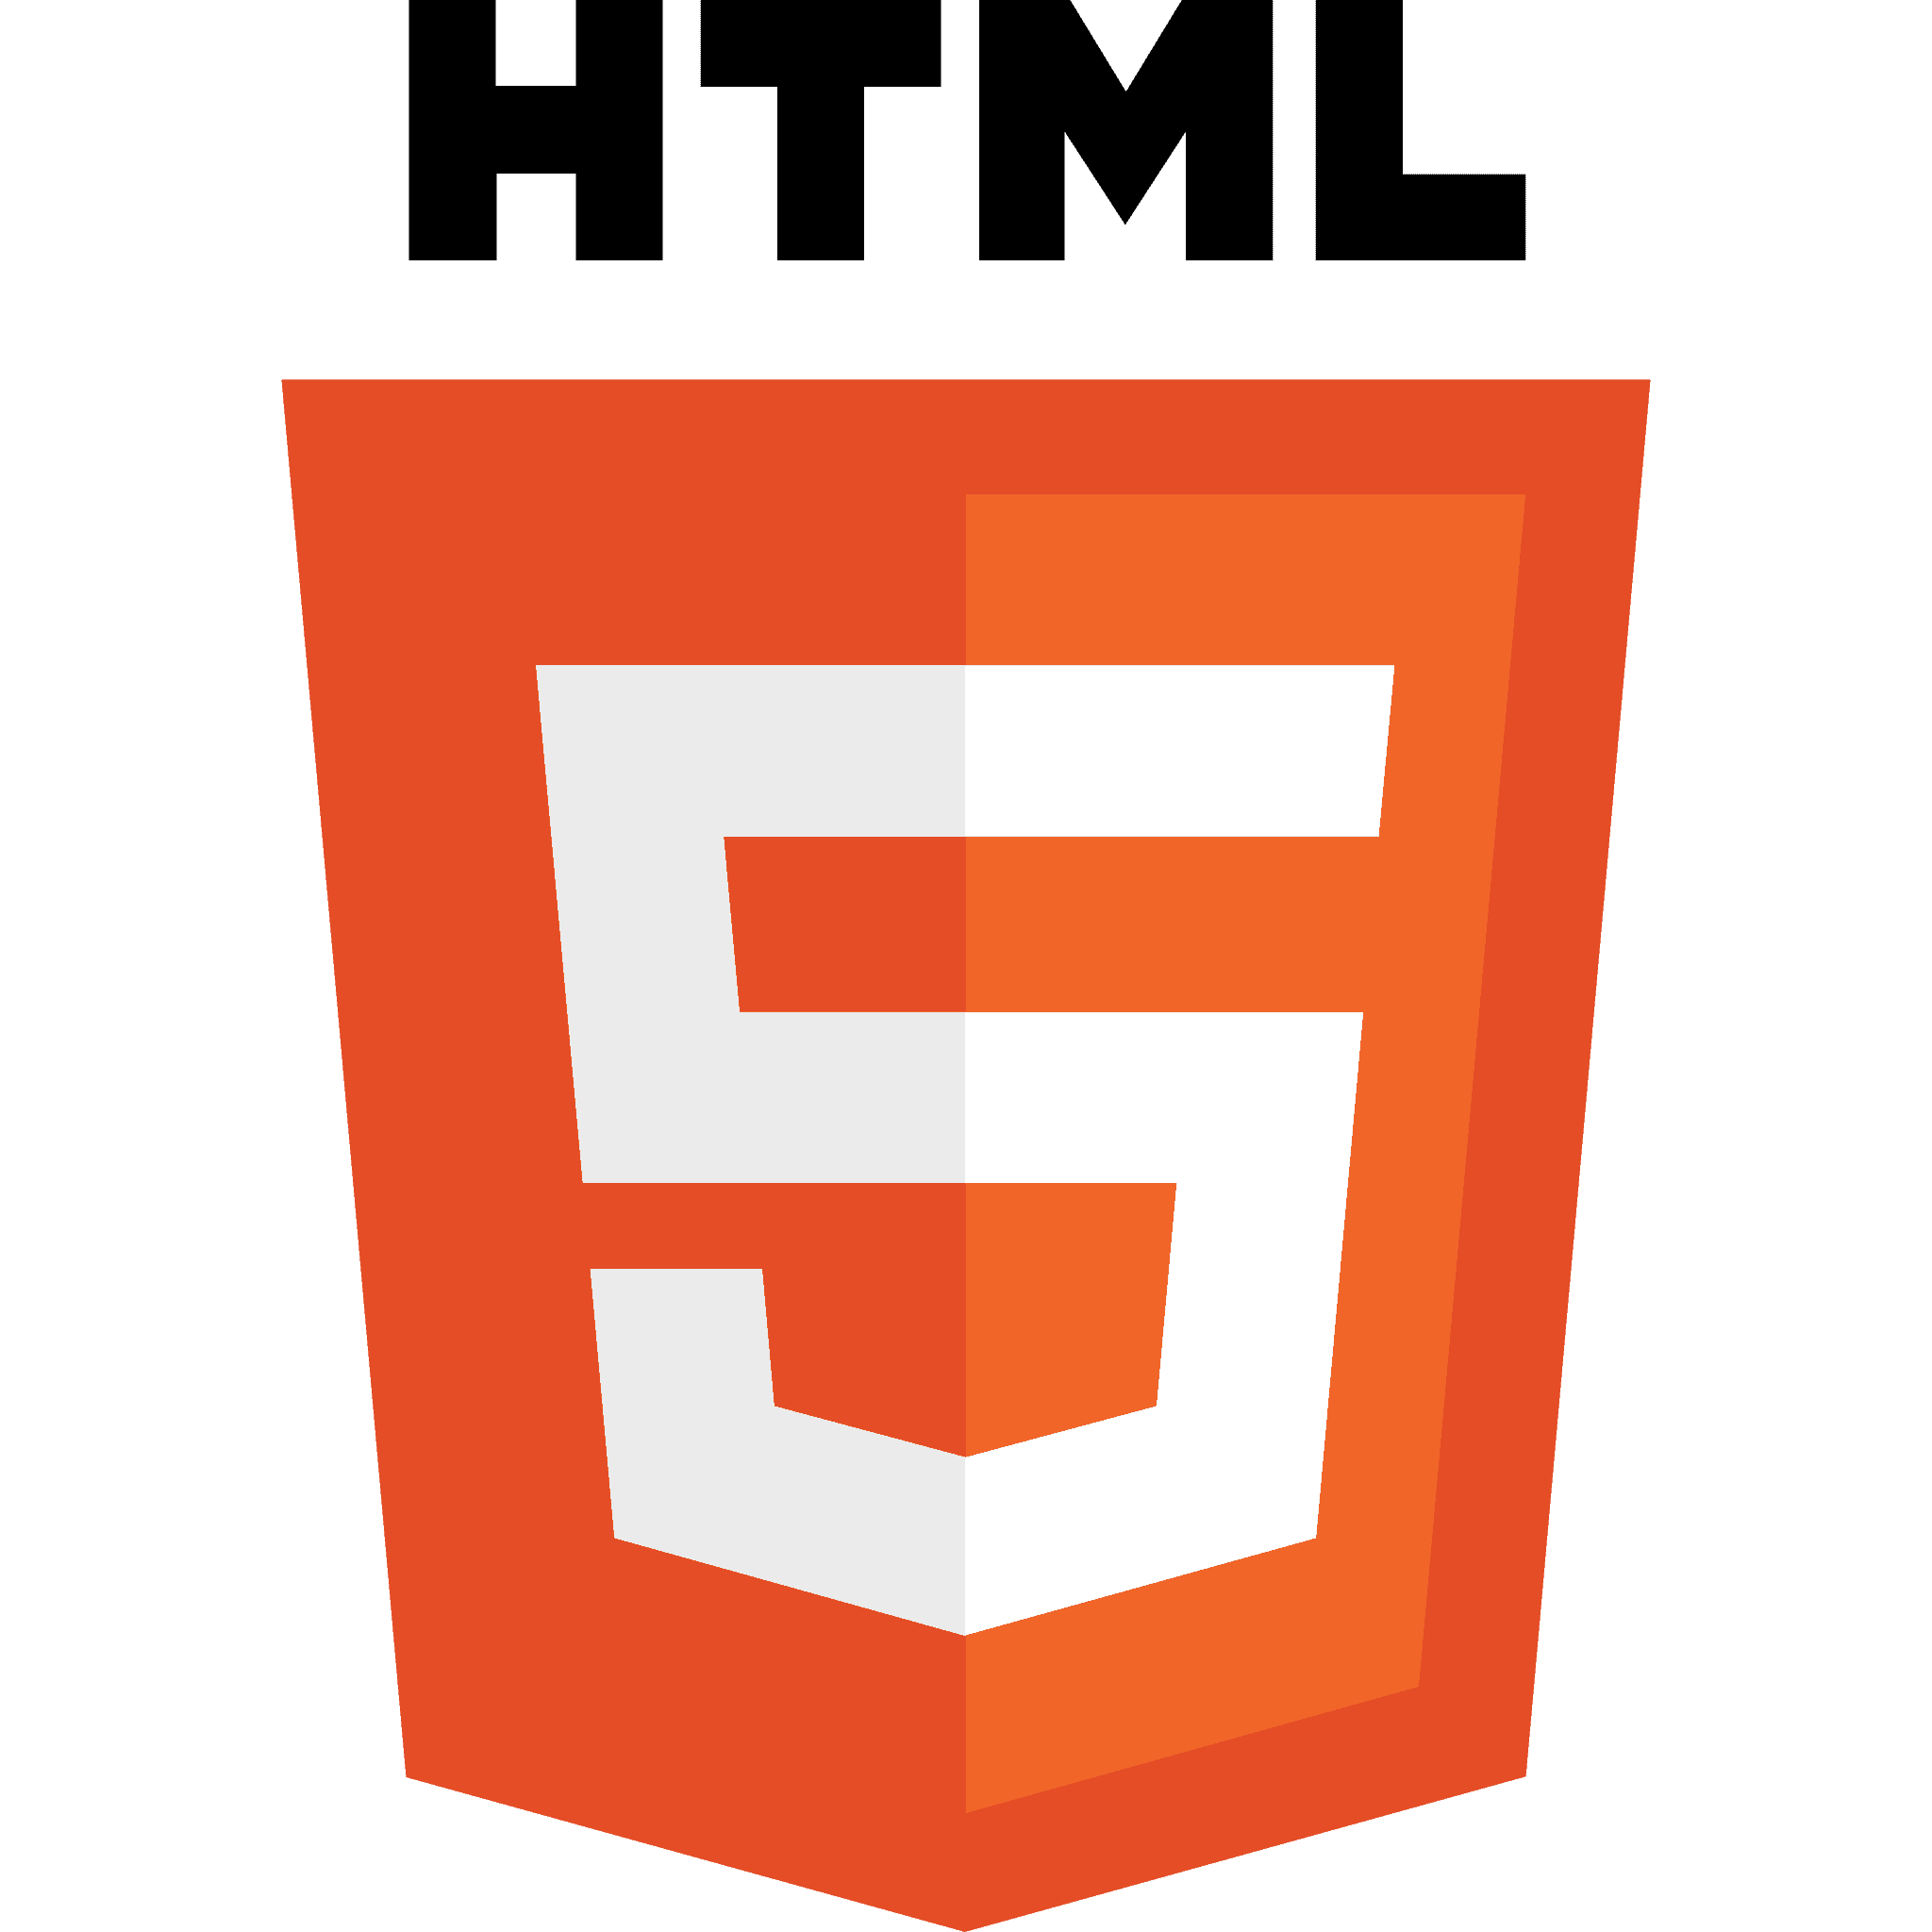
\includegraphics[width=0.5\textwidth]{img/html.png}
    \caption{HTML}
    \label{fig:html}
\end{figure}

\subsection{CSS}
CSS \cite{web:css} ย่อมาจาก Cascading Style Sheet  มักเรียกโดยย่อว่า "สไตล์ชีต" คือภาษาที่ใช้เป็นส่วนของการจัดรูปแบบการแสดงผลเอกสาร  HTML โดยที่ CSS กำหนดกฏเกณฑ์ในการระบุรูปแบบ (หรือ "Style") ของเนื้อหาในเอกสาร อันได้แก่ สีของข้อความ สีพื้นหลัง ประเภทตัวอักษร และการจัดวางข้อความ ซึ่งการกำหนดรูปแบบ หรือ Style นี้ใช้หลักการของการแยกเนื้อหาเอกสาร HTML ออกจากคำสั่งที่ใช้ในการจัดรูปแบบการแสดงผล กำหนดให้รูปแบบของการแสดงผลเอกสาร ไม่ขึ้นอยู่กับเนื้อหาของเอกสาร เพื่อให้ง่ายต่อการจัดรูปแบบการแสดงผลลัพธ์ของเอกสาร HTML โดยเฉพาะในกรณีที่มีการเปลี่ยนแปลงเนื้อหาเอกสารบ่อยครั้ง หรือต้องการควบคุมให้รูปแบบการแสดงผลเอกสาร HTML มีลักษณะของความสม่ำเสมอทั่วกันทุกหน้าเอกสารภายในเว็บไซต์เดียวกัน  โดยกฏเกณฑ์ในการกำหนดรูปแบบ (Style) เอกสาร HTML ถูกเพิ่มเข้ามาครั้งแรกใน HTML 4.0  เมื่อปีพ.ศ. 2539 ในรูปแบบของ CSS level 1 Recommendations ที่กำหนดโดย องค์กร World Wide Web Consortium หรือ W3C
\subsection{TypeScript}
Typescript \cite{web:typescript} คือภาษา JavaScript ใน Version ที่ได้รับการ Upgrade สามารถทำงานบน Node.js Environment หรือ Web Browser ต่าง ๆ ที่มีการรองรับ ECMAScript 3 ขึ้นไป TypeScript เป็น Statically Compiled Language ที่ได้จัดเตรียมทั้ง Static Typing, Classes และ Interface ไว้ให้แล้ว ช่วยให้คุณสามารถเขียน Code ของ JavaScript ที่เรียบง่ายและ Clean ได้อย่างสะดวกขึ้น ดังนั้น การใช้ TypeScript จะช่วยให้คุณสามารถสร้าง Software ที่ปรับใช้งานได้ง่ายและมีประสิทธิภาพมากยิ่งขึ้น

\subsection{Tailwind CSS}
Tailwind CSS \cite{web:tailwind} คือ CSS \cite{web:css} Framework ตัวหนึ่งที่มีรูปแบบการทำงานแบบ Utility-First โดย Utility คือ Class Selector ตัวหนึ่ง ที่เมื่อใช้งานก็เพียงเรียกใช้ Utility ต่างๆมาประกอบกันให้ได้การแสดงผลตามที่เราต้องการ ซึ่งจะมีความต่างกับ CSS Framework อื่นที่มักจะกำหนด Class Selector ให้เฉพาะเจาะจงกับรูปแบบการแสดงผลของ Element นั้น ๆ ไปเลย
\begin{figure}
    \centering
    
\includegraphics[width=0.5\textwidth]{img/tailwind.jpg}
    \caption{Tailwind CSS}
    \label{fig:tailwind}
\end{figure}
\subsection{Next.js}
Next.js \cite{web:nextjs} เป็น open-source React framework ซึ่งต่างจาก React ตรงที่ Next.js เป็นการใช้ server side rendering และยังสามารถทำเว็ปไซต์ได้ทั้งแบบ static และ dynamic ซึ่งข้อดีของการเป็น Server Side Rendering คือ ช่วยในเรื่อง SEO หรือ search engine optimization เพราะถ้าทำการ inspect เว็ปไซต์ที่สร้างโดย Next.js จะเห็นว่า source จะเป็น html ซะส่วนใหญ่ ซึ่งทำให้ SEO ค้นผ่าน source เพื่อให้ได้ข้อมูลและจัดหมวดหมู่ได้ง่ายกว่า React ที่เป็น JavaScript มากกว่า ทำให้ Next.js เป็นที่นิยมในหลาย ๆ บริษัท นอกจากนี้ ข้อดีก็คือ render ได้เร็วกว่า React เพราะ Next.js มีสิ่งที่เรียกว่า get static path ซึ่งการสร้าง path แบบ static แบบเว็ปไซต์ html โดยไม่ต้องทำการเชื่อมต่อกับ back-end เพื่อให้ได้ data ยิ่งไปกว่านั้น Next.js สามารถรวมเข้ากับ back-end ได้ง่ายๆ เพราะ Next.js มีสิ่งที่เรียกว่า API routes ในการรับส่ง request ใน folder ของ page จะมีอีก folder ที่เรียกว่า api ที่ถูกปฏิบัติเป็น endpoint แทนที่จะเป็น page ซึ่ง folder api นี้จะเป็นในส่วนหนึ่งของ server-side เท่านั้น ทำให้ไม่ไปเพิ่ม size ของ Client Side
\begin{figure}
    \centering
    
\includegraphics[width=0.5\textwidth]{img/nextjs.png}
    \caption{Next.js}
    \label{fig:nextjs}
\end{figure}
\subsection{MySQL}
MySQL \cite{web:mysql} คือ ระบบจัดการฐานข้อมูล หรือ Database Management System (DBMS) แบบข้อมูลเชิงสัมพันธ์ หรือ Relational Database Management System (RDBMS) ซึ่งเป็นระบบฐานข้อมูลที่จัดเก็บรวบรวมข้อมูลในรูปแบบตาราง โดยมีการแบ่งข้อมูลออกเป็นแถว (Row) และในแต่ละแถวแบ่งออกเป็นคอลัมน์ (Column) เพื่อเชื่อมโยงระหว่างข้อมูลในตารางกับข้อมูลในคอลัมน์ที่กำหนด แทนการเก็บข้อมูลที่แยกออกจากกัน โดยไม่มีความเชื่อมโยงกัน ซึ่งประกอบด้วยข้อมูล (Attribute) ที่มีความสัมพันธ์เชื่อมโยงกัน (Relation) โดยใช้ RDBMS Tools สำหรับการควบคุมและจัดเก็บฐานข้อมูลที่จำเป็น ทำให้นำไปประยุกต์ใช้งานได้ง่าย ช่วยเพิ่มประสิทธิภาพในการทำงานให้มีความยืดหยุ่นและรวดเร็วได้มากยิ่งขึ้น รวมถึงเชื่อมโยงข้อมูล ที่จัดแบ่งกลุ่มข้อมูลแต่ละประเภทได้ตามต้องการ จึงทำให้ MySQL เป็นโปรแกรมระบบจัดฐานข้อมูลที่ได้รับความนิยมสูง

% \subsection{Docker}

\subsection{JSON}
JSON \cite{web:json} ย่อมาจาก (JavaScript Object Notation) เป็นมาตรฐานในการแลกเปลี่ยนข้อมูล (Data Interchange Format) ที่ได้รับความนิยมแทบจะสูงที่สุดในปัจจุบัน ก่อกำเนิดขึ้นในช่วงต้นยุค 2000 ซึ่ง JSON เป็นที่นิยมโดยเฉพาะในงานด้านการทำ APIs ซึ่งเหล่า developers ทุกคนคงรู้จักและคุ้นเคยกันเป็นอย่างดี แม้ว่าจะมีรูปแบบข้อมูลอื่น ๆ อีกมากมายเช่น XML, CSV, YAML, etc เป็นต้น
\subsubsection{จุดเด่นของ JSON}
\begin{itemize}
    \item อ่านทำความเข้าใจได้ง่าย
    \item มีความเบา (lightweight)
    \item มีความเป็นมาตรฐานสูง และเป็นที่นิยมสูง
    \item มีความเร็วในการ access ข้อมูลที่สูง เพราะไม่ได้มีโครงสร้างที่ซับซ้อนเหมือนเช่น XML เป็นต้น
\end{itemize}


% \subsection{Relational Database Management System (RDBMS)}



\section{ด้าน User Interface}
ในส่วนนี้จะอธิบายถึงการออกแบบ User Interface ของเว็บแอปพลิเคชัน

\subsection{Design Thinking}
กระบวนการออกแบบ design thinking นั้นมีหลากหลายรูปแบบ ทั้งรูปแบบ 3 ขั้น ไปจนถึง 7 ขั้น ทุกรูปแบบมีความคล้ายคลึงมากที่สุด และใช้หลักการเดียวกันที่อ้างอิงจาก Herbert Simon ผู้ชนะรางวัลโนเบลในสาขา The Sciences of the Artificial ในปี 1969 โดยรูปแบบที่นิยมใช้กันมากที่สุด คือ รูปแบบของ Hasso-Plattner Institute of Design at Stanford มีทั้งหมด 5 กระบวนด้วยกัน ดังนี้
\begin{enumerate}
    \item Empathise หรือ การเข้าใจปัญหา
          คือ การทำความเข้าใจกับปัญหาก่อน ตั้งแต่การเข้าใจผู้ใช้ กลุ่มเป้าหมาย หรือเข้าใจสิ่งที่ต้องการแก้ไขเพื่อหาหนทางที่เหมาะสม และดีที่สุดให้ได้ โดยเริ่มต้นจาก การเข้าใจคำถาม สร้างสมมติฐาน กระตุ้นให้เกิดการใช้ความคิดที่นำไปสู่ความคิด สร้างสรรค์ และวิเคราะห์ปัญหาให้ถี่ถ้วน เพื่อหาแนวทางที่ชัดเจน นำไปสู่การแก้ไขปัญหาที่ตรงประเด็น และสร้างผลลัพธ์ที่ดีที่สุด
    \item Define หรือ กำหนดปัญหาให้ชัดเจน
          คือ การเข้าใจความต้องการ ปัญหา และวิเคราะห์ข้อมูลเชิงลึก เพื่อคัดกรองหาปัญหาที่แท้จริง กำหนดหรือบ่งชี้ปัญหาอย่างชัดเจน เพื่อที่จะเป็นแนวทางในการปฎิบัติ และมีทิศทางในการแก้ไขปัญหาอย่างชัดเจน
    \item Ideate หรือ ระดมความคิด
          คือ การนำเสนอแนวคิดต่างๆร่วมกัน ถึงวิธีการแก้ไขปัญหา อย่างไม่มีกรอบจำกัด การระดมความคิดควรมีมุมมองหลากหลาย และมีหลากหลายแนวทางให้ได้มากที่สุด เพื่อให้มีฐานข้อมูลในการนำไปวิเคราะห์และสรุปผล เพื่อนำไปแก้ไขปัญหา โดยไม่จำเป็นต้องเป็นแนวทางใดแนวทางหนึ่ง และการระดมความคิดยังช่วยมองให้เห็นปัญหาที่หลากหลายได้มากขึ้น
    \item Prototype หรือ สร้างต้นแบบที่เลือก
          คือ การออกแบบผลิตภัณฑ์หรือนวัตกรรม เพื่อสร้างต้นแบบสำหรับการทดสอบ และนำไปใช้จริง ซึ่งคือ การลงมือปฎิบัติหรือทดลองตามแนวทางการแก้ไขปัญหาที่ได้กำหนดไว้
    \item Test หรือ ทดสอบการแก้ไขปัญหา นํา Prototype ที่เราทําการทําขึ้นมาไปทดสอบกับผู้ใช้ว่าสามารถแก้ไขปัญหาของ
          ผู้ใช้ได้หรือไม่ และหลังจากนั้นถ้าหากการแก้ปัญหายังไม่สามารถช่วยแก้ไขได้
          หรือแก้ไขได้ยังไม่ดีพอ ผู้จัดทําจะต้องกลับไปทําตั้งแต่ขั้นตอนแรกอีกครั้งจนกว่าจะสามารถออกแบบโปรแกรมที่แก้ไขปัญหา
          ของผู้ใช้ได้


          \begin{figure}
              \begin{center}
                  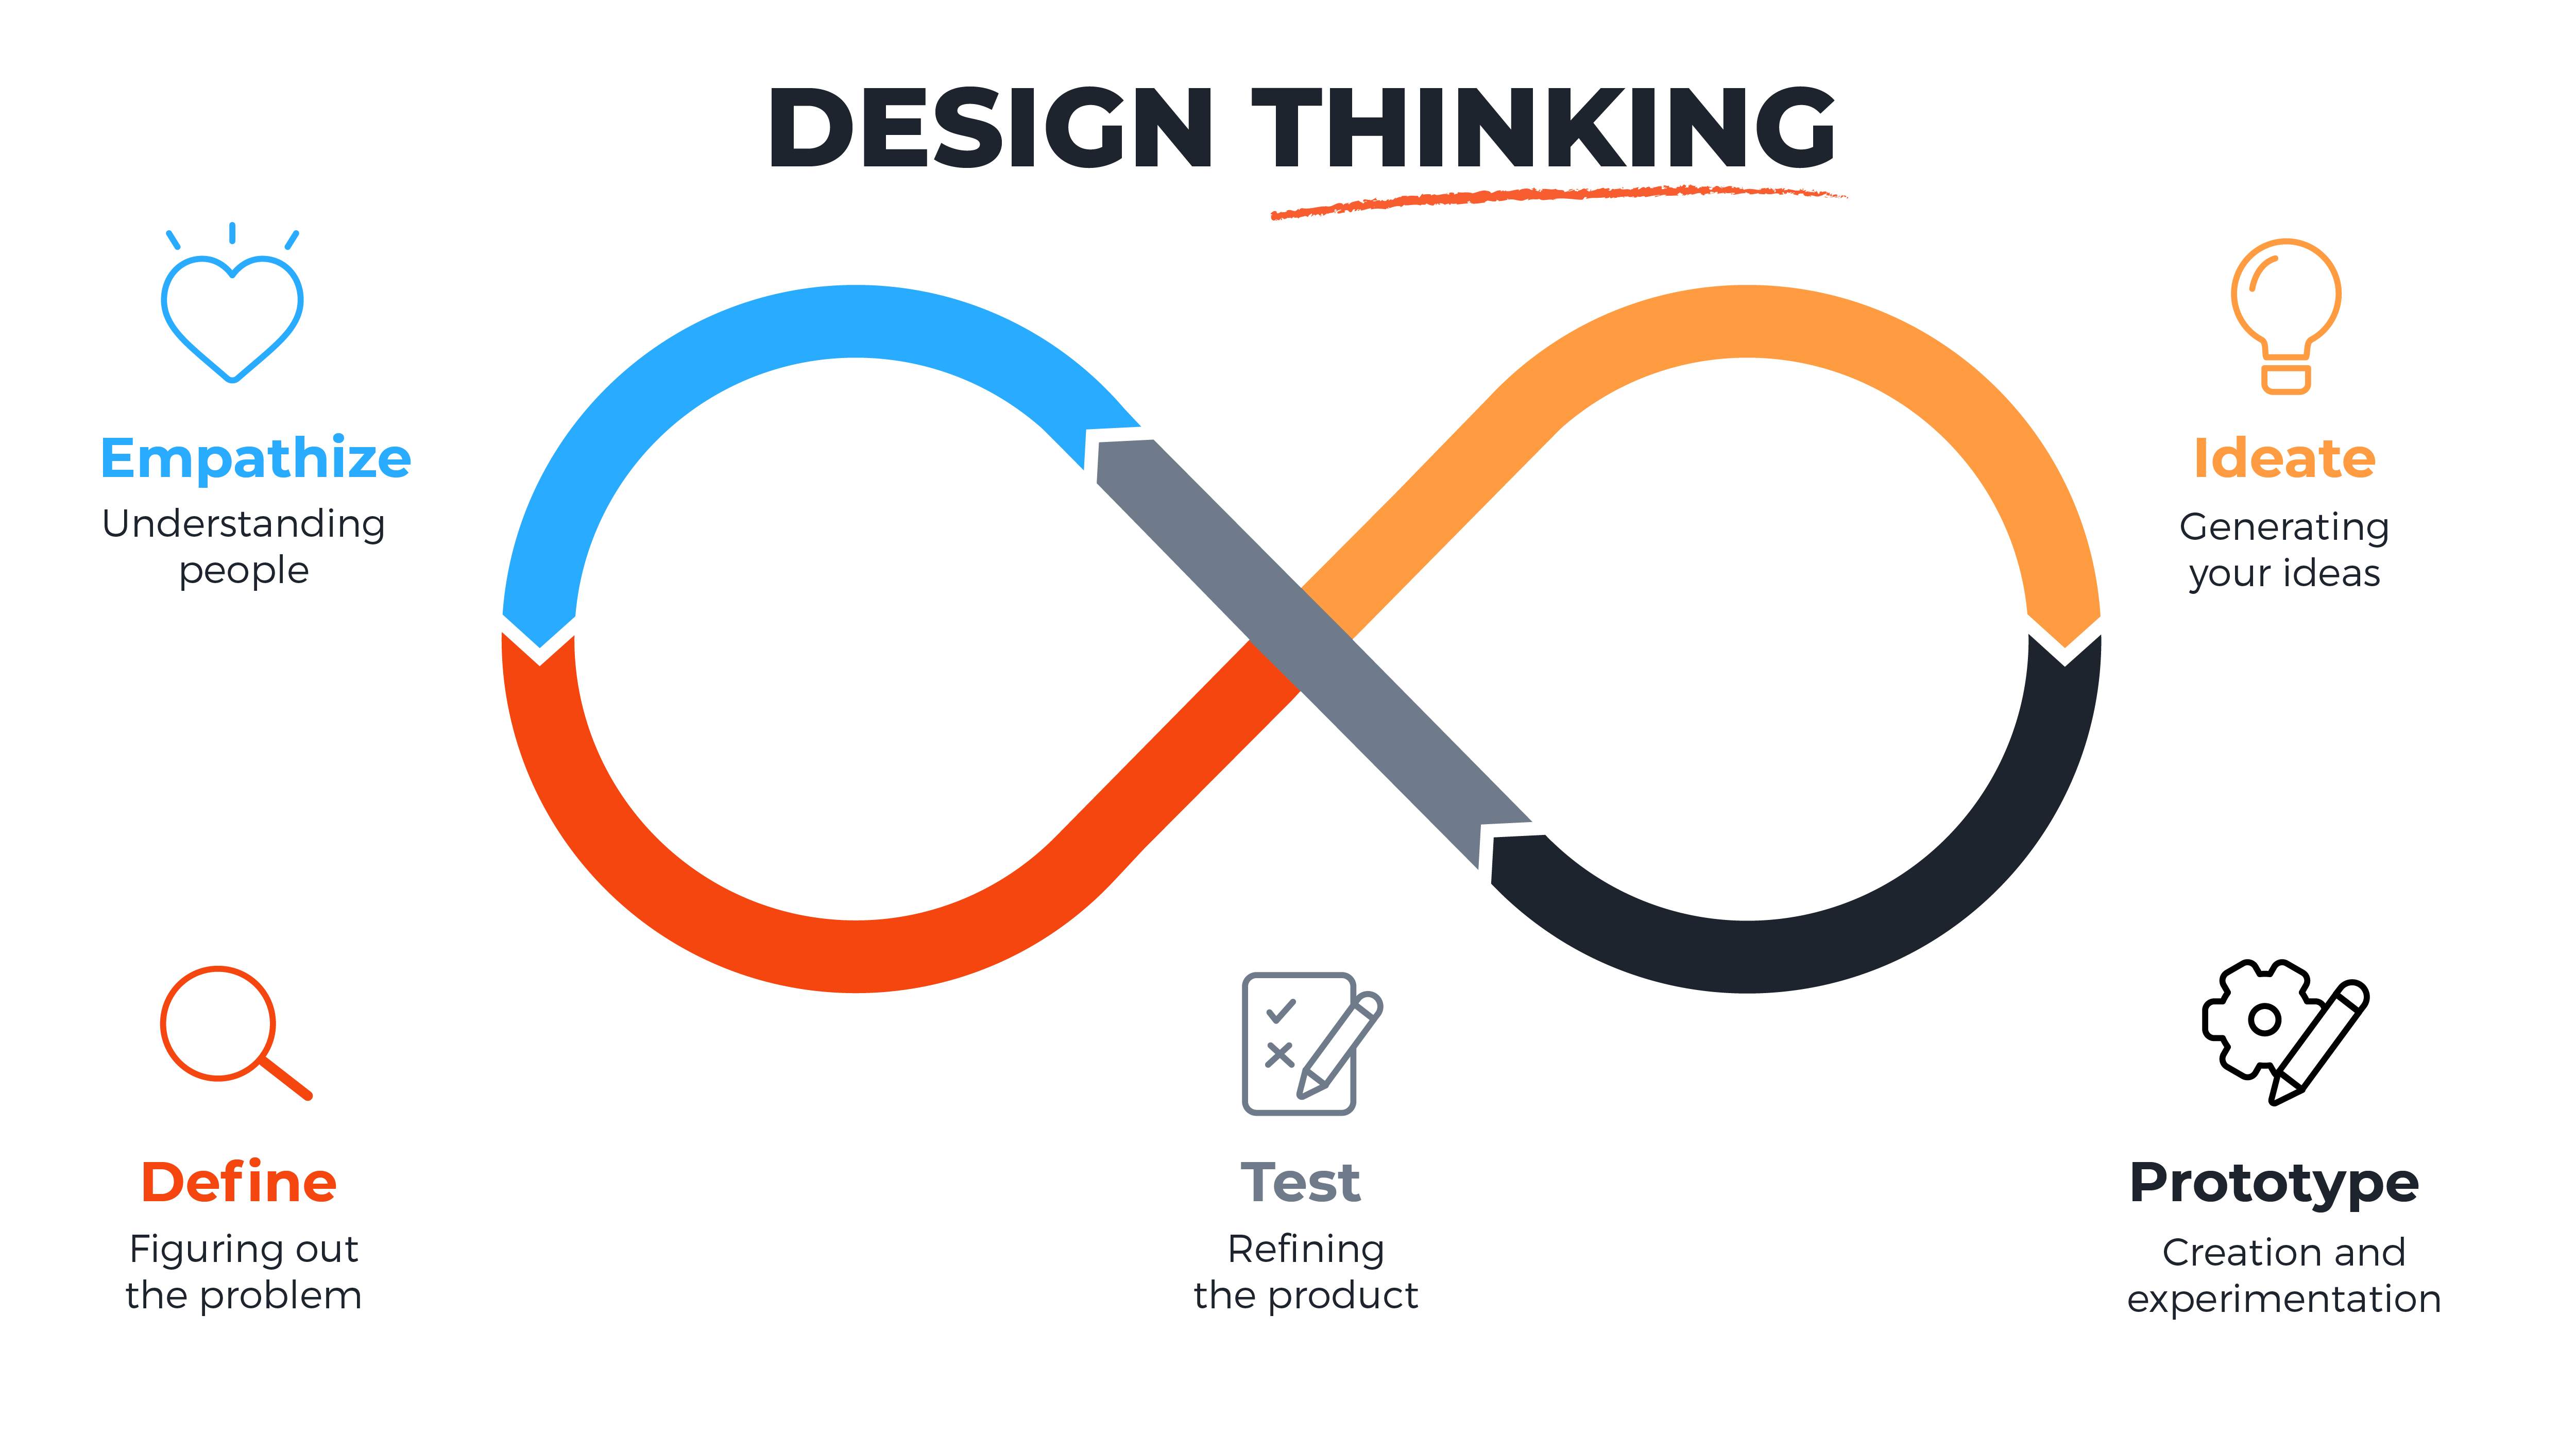
\includegraphics[width=0.8\textwidth]{img/design-thinking.png}
              \end{center}
              \caption[Poem]{กระบวนการออกแบบ Design Thinking}
              \label{fig:design-thinking}
          \end{figure}

\end{enumerate}


% \noindent
% where $\omega$ is the frequency of the plasmon, $c$ is the speed of
% light, $\varepsilon_m$ is the dielectric constant of the metal,
% $\varepsilon_i$ is the dielectric constant of neighboring insulator,
% and $\varepsilon_\mathit{air}$ is the dielectric constant of air.

% \section{About using figures in your report}

% % define a command that produces some filler text, the lorem ipsum.
% \newcommand{\loremipsum}{
%   \textit{Lorem ipsum dolor sit amet, consectetur adipisicing elit, sed do
%   eiusmod tempor incididunt ut labore et dolore magna aliqua. Ut enim ad
%   minim veniam, quis nostrud exercitation ullamco laboris nisi ut
%   aliquip ex ea commodo consequat. Duis aute irure dolor in
%   reprehenderit in voluptate velit esse cillum dolore eu fugiat nulla
%   pariatur. Excepteur sint occaecat cupidatat non proident, sunt in
%   culpa qui officia deserunt mollit anim id est laborum.}\par}

% \begin{figure}
%   \centering

%   \fbox{
%      \parbox{.6\textwidth}{\loremipsum}
%   }

%   % To include an image in the figure, say myimage.pdf, you could use
%   % the following code. Look up the documentation for the package
%   % graphicx for more information.
%   % \includegraphics[width=\textwidth]{myimage}

%   \caption[Sample figure]{This figure is a sample containing \gls{lorem ipsum},
%   showing you how you can include figures and glossary in your report.
%   You can specify a shorter caption that will appear in the List of Figures.}
%   \label{fig:sample-figure}
% \end{figure}

% Using \verb.\label. and \verb.\ref. commands allows us to refer to
% figures easily. If we can refer to Figures
% \ref{fig:walrus} and \ref{fig:sample-figure} by name in the {\LaTeX}
% source code, then we will not need to update the code that refers to it
% even if the placement or ordering of the figures changes.

% \loremipsum\loremipsum

% % This code demonstrates how to get a landscape table or figure. It
% % uses the package lscape to turn everything but the page number into
% % landscape orientation. Everything should be included within an
% % \afterpage{ .... } to avoid causing a page break too early.
% \afterpage{
%   \begin{landscape}
%   \begin{table}
%     \caption{Sample landscape table}
%     \label{tab:sample-table}

%     \centering

%     \begin{tabular}{c||c|c}
%         Year & A & B \\
%         \hline\hline
%         1989 & 12 & 23 \\
%         1990 & 4 & 9 \\
%         1991 & 3 & 6 \\
%     \end{tabular}
%   \end{table}
%   \end{landscape}
% }

% \loremipsum\loremipsum\loremipsum

% \section{Overfull hbox}

% When the \verb.semifinal. option is passed to the \verb.cpecmu. document class,
% any line that is longer than the line width, i.e., an overfull hbox, will be
% highlighted with a black solid rule:
% \begin{center}
% \begin{minipage}{2em}
% juxtaposition
% \end{minipage}
% \end{center}

\section{\ifenglish%
      \ifcpe CPE \else ISNE \fi knowledge used, applied, or integrated in this project
  \else%
      ความรู้ตามหลักสูตรซึ่งถูกนำมาใช้หรือบูรณาการในโครงงาน
  \fi
 }

\begin{itemize}
    \item 261207 Basic CPE Lab นําความรู้ทางด้านการพัฒนาเว็บแอพพลิเคชัน เช่น HTML, CSS, Tailwind CSS, JavaScript, TypeScript, Next.js
          และ Node.js มาใช้ในการพัฒนาเว็บแอพพลิเคชัน ทั้งด้านของ front-end ซึ่งจะแสดงผลของเว็บไซต์ และ back-end ที่จะจัดการการทำงานต่าง ๆ รวมถึงการเชื่อมต่อกับฐานข้อมูล
    \item 261361 Software Engineering การใช้กระบวนการทางวิศวกรรมในการดูแลการผลิต ตั้งแต่การเริ่มเก็บความต้องการ การตั้งเป้าหมายของระบบ การออกแบบ กระบวนการพัฒนา การตรวจสอบ การประเมินผลและทดสอบระบบ
    \item 261346 Database Systems การใช้งานฐานข้อมูล โดยใช้ MySQL ในการจัดการฐานข้อมูล รวมถึงการเชื่อมต่อกับฐานข้อมูล
          และการเขียนคำสั่ง SQL ในการดึงข้อมูลจากฐานข้อมูลและการจัดการข้อมูลในฐานข้อมูล
    \item 261

          % \item 261102 Computer Programming การเขียน ทดสอบ และดูแลซอร์สโค้ดของโปรแกรมคอมพิวเตอร์
          %       ซึ่งซอร์สโค้ดนั้นจะเขียนด้วยภาษาโปรแกรม ขั้นตอนการเขียนโปรแกรมต้องการความรู้ในหลายด้านด้วยกัน
          %       รวมถึงการนํา GitHub มาใช้ในการเขียนโปรแกรม
\end{itemize}

% อธิบายถึงความรู้ และแนวทางการนำความรู้ต่างๆ ที่ได้เรียนตามหลักสูตร ซึ่งถูกนำมาใช้ในโครงงาน

\section{\ifenglish%
      Extracurricular knowledge used, applied, or integrated in this project
  \else%
      ความรู้นอกหลักสูตรซึ่งถูกนำมาใช้หรือบูรณาการในโครงงาน
  \fi
 }

% อธิบายถึงความรู้ต่างๆ ที่เรียนรู้ด้วยตนเอง และแนวทางการนำความรู้เหล่านั้นมาใช้ในโครงงาน

\chapter{\ifproject%
      \ifenglish Project Structure and Methodology\else โครงสร้างและขั้นตอนการทำงาน\fi
  \else%
      \ifenglish Project Structure\else โครงสร้างของโครงงาน\fi
  \fi
 }

ในบทนี้จะกล่าวถึงหลักการ และการออกแบบระบบ

\makeatletter

% \renewcommand\section{\@startsection {section}{1}{\z@}%
%                                    {13.5ex \@plus -1ex \@minus -.2ex}%
%                                    {2.3ex \@plus.2ex}%
%                                    {\normalfont\large\bfseries}}

\makeatother
%\vspace{2ex}
% \titleformat{\section}{\normalfont\bfseries}{\thesection}{1em}{}
% \titlespacing*{\section}{0pt}{10ex}{0pt}

\section{หลักการทำงานของระบบ}


% \begin{figure}
% \begin{center}
% \includegraphics{800px-Briny_Beach.jpg}
% \end{center}
% \caption[Poem]{The Walrus and the Carpenter}
% \label{fig:walrus}
% \end{figure}
\subsection{การทำงานของระบบ (System Architecture)}
\begin{figure}[h]
    \begin{center}
        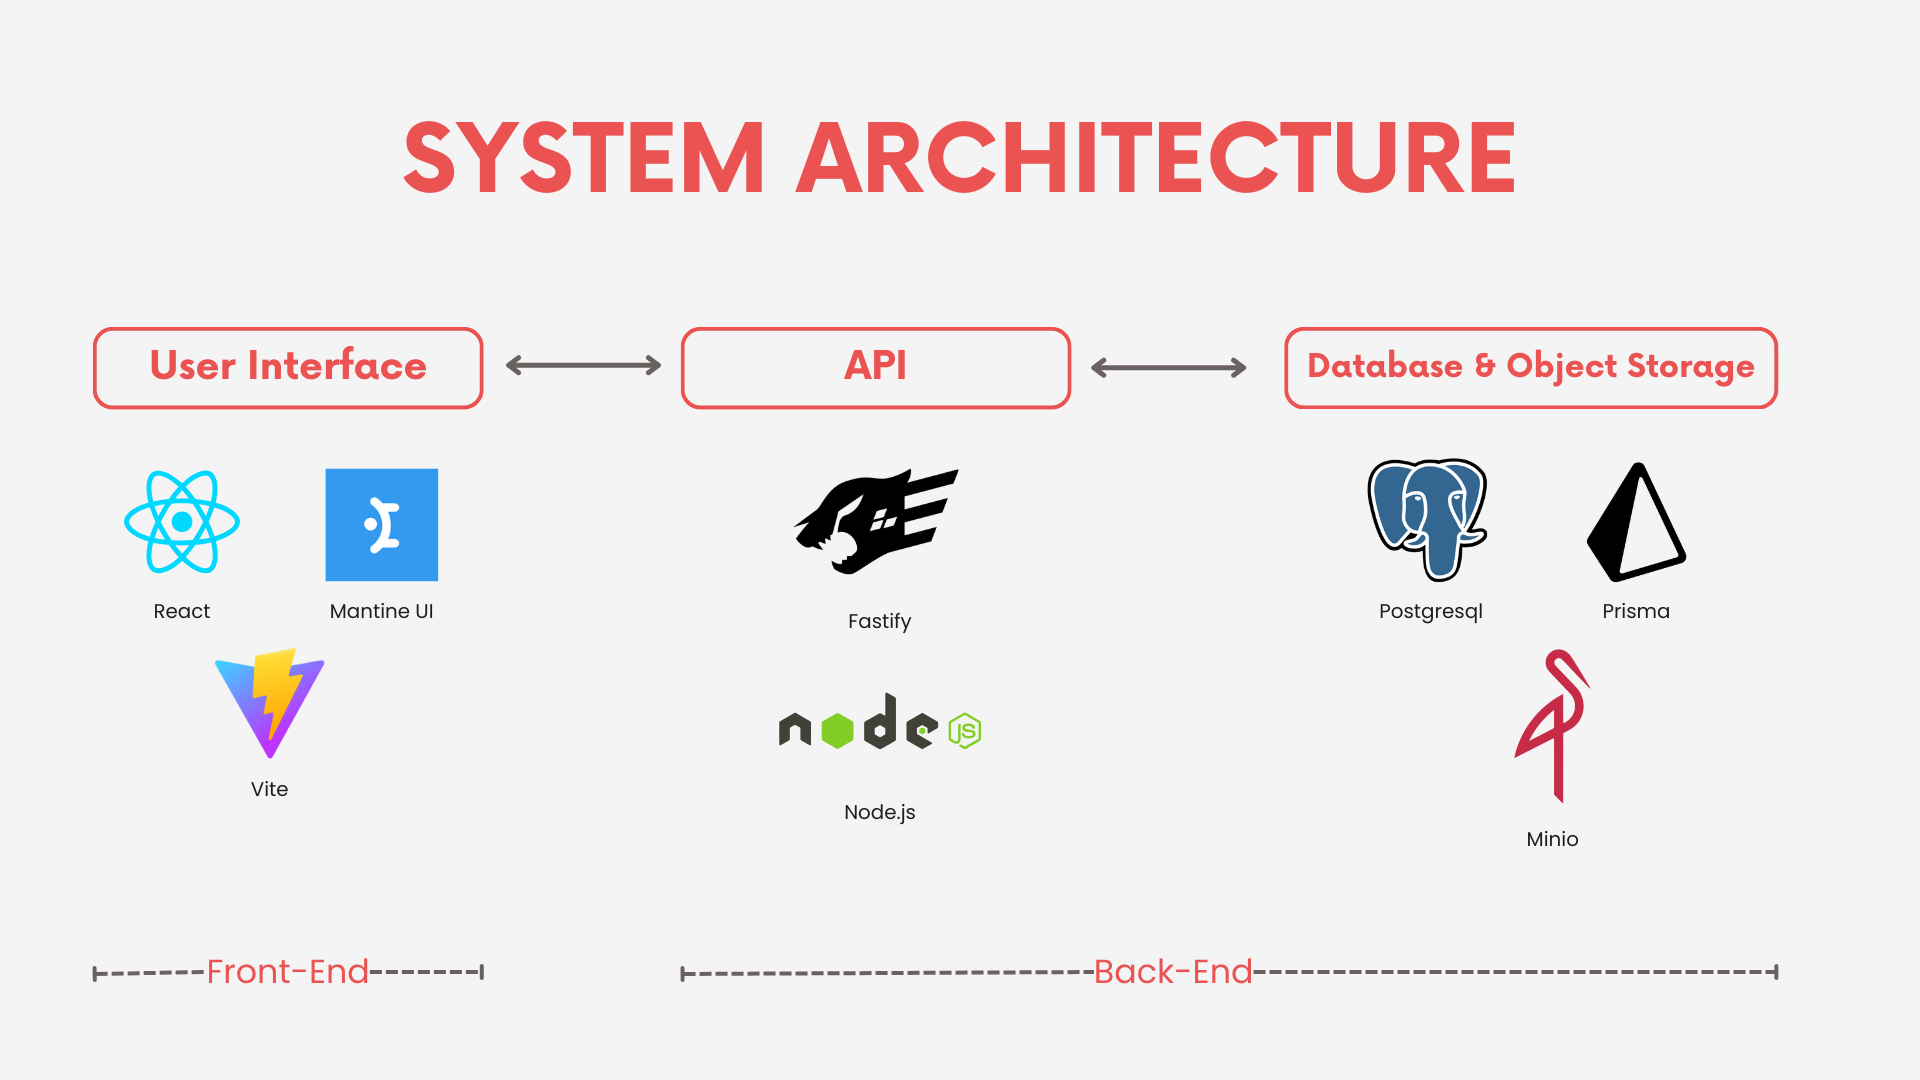
\includegraphics[width=0.9\textwidth]{img/system achitecture.png}
    \end{center}
    \caption{System Architecture}
    \label{fig:system_overview}
\end{figure}

จากรูปที่ \ref{fig:system_overview} จะเป็นภาพรวมของระบบที่เราได้ทำการออกแบบขึ้น โดยมีรายละเอียดดังนี้
\begin{itemize}
    \item Frontend

          ส่วนหน้าบ้าน (Frontend) เป็นส่วนการพัฒนาเพื่อแสดง User Interface (UI) โดยโครงการนี้ได้ใช้เทคโนโลยี React ร่วมกับ Mantine UI ในการออกแบบและสร้างส่วนติดต่อผู้ใช้ (UI) โดยมีหน้าที่แสดงผลลัพธ์ต่อผู้ใช้ในรูปแบบที่เข้าใจง่าย รับข้อมูลป้อนจากผู้ใช้ผ่านอินเทอร์เฟซต่าง ๆ เช่น ปุ่ม ฟิลด์ข้อความ ฯลฯ และสื่อสารกับ API เพื่อส่งคำร้องขอและรับผลลัพธ์
    \item Backend

          ส่วนหลังบ้าน (Backend) เป็นส่วนที่ทำหน้าที่รับข้อมูลจากผู้ใช้ จากนั้นทำการประมวลผลข้อมูล และส่งข้อมูลกลับไปยังผู้ใช้ โดยโครงการนี้ได้ใช้เทคโนโลยี Fastify เว็บเฟรมเวิร์ค Node.js ร่วมกับ Prisma ORM ในการจัดการข้อมูลในฐานข้อมูล รวมถึงทำการสื่อสารกับฐานข้อมูล PostgreSQL และ Minio (Object Storage) ในการจัดการข้อมูลที่เป็นไฟล์
\end{itemize}

\subsection{เส้นทางของผู้ใช้ (User Flow)}
\begin{figure}[h]
    \begin{center}
        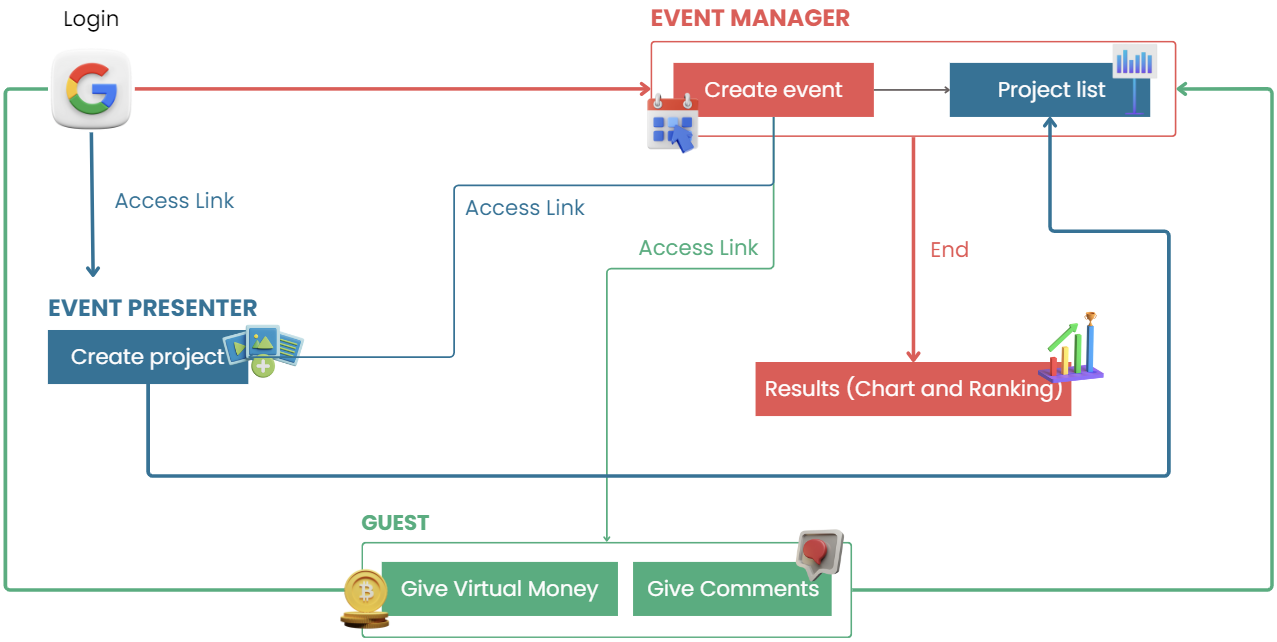
\includegraphics[width=0.9\textwidth]{img/userflow.png}
    \end{center}
    \caption{User Flow}
    \label{fig:user_flow}
\end{figure}

จากรูปที่ \ref{fig:user_flow} จะเป็นเส้นทางของผู้ใช้งานที่เข้าใช้งานระบบ โดยมีรายละเอียดดังนี้

\subsubsection{ผู้สร้างงานกิจกรรม (Event Manager)}
\begin{itemize}
    \item ผู้ใช้เข้าสู่ระบบโดยใช้ Google Account
    \item ผู้ใช้สร้าง Event ใหม่ โดยป้อนข้อมูลต่าง ๆ เช่น ชื่องานกิจกรรม รายละเอียด วันเวลา สถานที่ เป็นต้น
    \item ผู้ใช้สร้าง Event เสร็จสิ้น จะมี QR Code หรือ Access Link สำหรับนำไปให้ผู้นำเสนอโครงการ (Presenter) สำหรับเพิ่มโครงการและผู้เข้าร่วมกิจกรรม (Guest) สำหรับเข้าร่วมกิจกรรม
    \item ผู้ใช้สามารถดูผลลัพธ์ (Chart และ Ranking) ของโครงการต่าง ๆ ที่เข้าร่วมกิจกรรมในระหว่างจัดงานกิจกรรม

\end{itemize}

\subsubsection{ผู้นำเสนอโครงการ (Presenter)}
\begin{itemize}
    \item ผู้ใช้เข้าสู่ระบบโดยใช้ Google Account
    \item ผู้ใช้สร้าง Project ใหม่ โดยป้อนข้อมูลต่าง ๆ เช่น ชื่อโครงการ รายละเอียด รูปภาพ ลิงก์ และไฟล์อื่น ๆ ที่เกี่ยวข้อง
    \item ผู้ใช้ดูผลลัพธ์ว่าโครงการได้รับ Virtual Money จากผู้เข้าร่วมกิจกรรม (Guest) และความคิดเห็นเกี่ยวกับโครงการหลังจากเสร็จสิ้นงานกิจกรรม

\end{itemize}

\subsubsection{ผู้เข้าร่วมกิจกรรม (Guest)}
\begin{itemize}
    \item ผู้ใช้เข้าร่วม Event โดยใช้ QR Code หรือ Access Link ที่ได้รับจาก Event Manager
    \item ผู้ใช้เข้าสู่ระบบโดยใช้ Google Account
    \item ผู้ใช้ดูรายละเอียดของงานกิจกรรมที่จัดขึ้น รวมถึงโครงการที่เข้าร่วมกิจกรรม
    \item ผู้ใช้สามารถให้ Virtual Money และแสดงความคิดเห็นเกี่ยวกับ Project ต่าง ๆ ที่เข้าร่วมกิจกรรมได้
\end{itemize}

\newpage
\subsection{โครงสร้างฐานข้อมูล (Database Schema)}
\begin{center}
    \begin{figure*}[h]
        \centering
        \includegraphics[width=1.0\textwidth]{img/database schama.png}
        \caption{Database Schema}
        \label{fig:data_schema}
    \end{figure*}
\end{center}
จากรูปที่ \ref{fig:data_schema} จะเป็นโครงสร้างของฐานข้อมูลที่ใช้ในระบบ โดยมีทั้งหมด 9  ตาราง ดังนี้
\begin{itemize}
    \item \textbf{Users} ใช้เก็บข้อมูลผู้ใช้งาน โดยจะเก็บข้อมูลผู้ที่เป็นผู้จัดงานกิจกรรมและผู้นำเสนอโครงการ ซึ่งผู้ใช้งาน 1 คนสามารถเป็นได้ทั้งผู้จัดงานกิจกรรมและผู้นำเสนอโครงการ
    \item \textbf{Events} ใช้เก็บข้อมูลงานกิจกรรม โดยจะเก็บข้อมูลเช่น ชื่องานกิจกรรม รายละเอียด วันเวลา สถานที่ และข้อมูลอื่น ๆ ที่เกี่ยวข้อง ซึ่ง 1 ผู้ใช้งานสามารถสร้างงานกิจกรรมได้หลายงานกิจกรรม
    \item \textbf{Projects} ใช้เก็บข้อมูลโครงการ โดยจะเก็บข้อมูลเช่น ชื่อโครงการ รายละเอียด รูปภาพ ลิงก์ และไฟล์อื่น ๆ ที่เกี่ยวข้อง ซึ่ง 1 ผู้ใช้งานสามารถสร้างโครงการได้หลายโครงการ
    \item \textbf{Virtual Money} ใช้เก็บข้อมูลเงินเสมือนที่โครงการได้รับ ซึ่ง 1 โครงการสามารถมีเงินเสมือนได้หลายรายการจากแขกผู้เข้าร่วมงาน
    \item \textbf{Guests} ใช้เก็บข้อมูลแขกผู้เข้าร่วมงาน ซึ่งจะเก็บข้อมูลทั่วไป และเก็บจำนวนเงินเสมือนที่มีอยู่ สำหรับให้โครงการต่าง ๆ
    \item \textbf{Thumbnails} ใช้เก็บข้อมูลรูปภาพ Thumbnail ของงานกิจกรรม โดย 1 งานกิจกรรมสามารถมี Thumbnail ได้เพียง 1 รูป
    \item \textbf{Documents} ใช้เก็บข้อมูลไฟล์เอกสารที่เกี่ยวข้องกับโครงการ ซึ่ง 1 โครงการสามารถมีไฟล์เอกสารได้หลายไฟล์
    \item \textbf{Comments} ใช้เก็บข้อมูลความคิดเห็นของแขกผู้เข้าร่วมงานที่มีต่อโครงการ ซึ่ง 1 โครงการสามารถมีความคิดเห็นได้หลายความคิดเห็น
    \item \textbf{Project Images} ใช้เก็บข้อมูลรูปภาพที่เกี่ยวข้องกับโครงการ ซึ่ง 1 โครงการสามารถมีรูปภาพได้หลายรูปภาพ
\end{itemize}

% \clearpage
\begin{table}[h]
    \centering
    \begin{tabular}{|l|c|l|}
        \hline
        ชื่อคอลัมน์               & ชนิดข้อมูล          & คำอธิบาย             \\ \hline
        \textbf{id}           & \textbf{INTEGER} & \textbf{รหัสผู้ใช้งาน} \\ \hline
        \verb |first_name_th| & VARCHAR          & ชื่อภาษาไทย          \\ \hline
        \verb |last_name_th|  & VARCHAR          & นามสกุลภาษาไทย      \\ \hline
        \verb |first_name_en| & VARCHAR          & ชื่อภาษาอังกฤษ        \\ \hline
        \verb |last_name_en|  & VARCHAR          & นามสกุลภาษาอังกฤษ    \\ \hline
        \verb |email|         & VARCHAR          & อีเมล               \\ \hline
        \verb |affiliation|   & TEXT             & สังกัด               \\ \hline
        \verb |profile_pic|   & TEXT             & รูปภาพโปรไฟล์        \\ \hline
        \verb |role|          & VARCHAR          & บทบาทของผู้ใช้งาน     \\ \hline
        \verb |created_at|    & TIMESTAMP        & วันที่สร้างข้อมูล        \\ \hline
        \verb |updated_at|    & TIMESTAMP        & วันที่อัปเดตข้อมูล       \\ \hline
    \end{tabular}
    \caption{ตารางข้อมูลผู้ใช้งาน (Users)}
    \label{tab:user_data}
\end{table}

\begin{table}[h]
    \centering
    \begin{adjustbox}{width=0.8\textwidth} % Add this line before \begin{tabular}
        \begin{tabular}{|l|c|l|}
            \hline
            ชื่อคอลัมน์                  & ชนิดข้อมูล          & คำอธิบาย                                 \\ \hline
            \textbf{id}              & \textbf{INTEGER} & \textbf{รหัสงานกิจกรรม}                  \\ \hline
            \verb |event_name|       & VARCHAR          & ชื่องานกิจกรรม                            \\ \hline
            \verb |start_date|       & DATE             & วันที่เริ่มงานกิจกรรม                        \\ \hline
            \verb |end_date|         & DATE             & วันที่สิ้นสุดงานกิจกรรม                       \\ \hline
            \verb |description|      & TEXT             & รายละเอียดงานกิจกรรม                     \\ \hline
            \verb |submit_start|     & DATE             & วันที่เริ่มรับส่งโครงการ                      \\ \hline
            \verb |submit_end|       & DATE             & วันที่สิ้นสุดรับส่งโครงการ                     \\ \hline
            \verb |number_of_member| & INTEGER          & จำนวนสมาชิกของโครงการ                    \\ \hline
            \verb |virtual_money|    & INTEGER          & จำนวนเงินเสมือนที่จะให้แขกผู้เข้าร่วมงาน (Guest) \\ \hline
            \verb |unit_money|       & VARCHAR          & หน่วยเงินเสมือนที่จะให้แขกผู้เข้าร่วมงาน (Guest) \\ \hline
            \verb |published|        & BOOLEAN          & สถานะการเผยแพร่ของงานกิจกรรม             \\ \hline
            \verb |organization|     & TEXT             & สังกัดของงานกิจกรรม                       \\ \hline
            \verb |video_link|       & TEXT             & ลิงก์วิดีโอที่เกี่ยวข้องกับงานกิจกรรม             \\ \hline
            \underline{user\_id}     & INTEGER          & รหัสผู้ใช้งานที่สร้างงานกิจกรรม                \\ \hline
            \verb |location|         & TEXT             & สถานที่จัดงานกิจกรรม                       \\ \hline
            \verb |created_at|       & TIMESTAMP        & วันที่สร้างข้อมูล                            \\ \hline
            \verb |updated_at|       & TIMESTAMP        & วันที่อัปเดตข้อมูล                           \\ \hline
        \end{tabular}
    \end{adjustbox} % Add this line after \end{tabular}
    \caption{ตารางข้อมูลงานกิจกรรม (Events)}
    \label{tab:event_data}
\end{table}

\begin{table}[h]
    \centering
    \begin{tabular}{|l|c|l|}
        \hline
        ชื่อคอลัมน์               & ชนิดข้อมูล          & คำอธิบาย                     \\ \hline
        \textbf{id}           & \textbf{INTEGER} & \textbf{รหัสโครงการ}        \\ \hline
        \verb |title|         & VARCHAR          & ชื่อโครงการ                  \\ \hline
        \verb |description|   & TEXT             & รายละเอียดของโครงการ        \\ \hline
        \underline{user\_id}  & INTEGER          & รหัสผู้ใช้งานที่สร้างโครงการ      \\ \hline
        \underline{event\_id} & INTEGER          & รหัสงานกิจกรรมที่โครงการเข้าร่วม \\ \hline
        \verb |created_at|    & TIMESTAMP        & วันที่สร้างข้อมูล                \\ \hline
    \end{tabular}
    \caption{ตารางข้อมูลโครงการ (Projects)}
    \label{tab:project_data}
\end{table}

\begin{table}[h]
    \centering
    \begin{tabular}{|l|c|l|}
        \hline
        ชื่อคอลัมน์                 & ชนิดข้อมูล          & คำอธิบาย                      \\ \hline
        \textbf{id}             & \textbf{INTEGER} & \textbf{รหัสโครงการที่ได้รับเงิน} \\ \hline
        \verb |amount|          & INTEGER          & จำนวนเงินเสมือนที่ได้รับ           \\ \hline
        \underline{project\_id} & INTEGER          & รหัสโครงการที่ได้รับเงิน          \\ \hline
        \underline{event\_id}   & INTEGER          & รหัสงานกิจกรรมที่ได้รับเงิน        \\ \hline
        \underline{guest\_id}   & INTEGER          & รหัสผู้เข้าร่วมกิจกรรมที่ได้รับเงิน    \\ \hline
        \verb |created_at|      & TIMESTAMP        & วันที่สร้างข้อมูล                 \\ \hline
        \verb |updated_at|      & TIMESTAMP        & วันที่อัปเดตข้อมูล                \\ \hline
    \end{tabular}
    \caption{ตารางข้อมูลเงินเสมือน (Virtual Money)}
    \label{tab:virtual_money_data}
\end{table}

\begin{table}[h]
    \centering
    \begin{tabular}{|l|c|l|}
        \hline
        ชื่อคอลัมน์               & ชนิดข้อมูล          & คำอธิบาย                    \\ \hline
        \textbf{id}           & \textbf{INTEGER} & \textbf{รหัสผู้เข้าร่วมกิจกรรม} \\ \hline
        \verb |first_name_th| & VARCHAR          & ชื่อจริงภาษาไทย              \\ \hline
        \verb |last_name_th|  & VARCHAR          & นามสกุลภาษาไทย             \\ \hline
        \verb |first_name_en| & VARCHAR          & ชื่อจริงภาษาอังกฤษ            \\ \hline
        \verb |last_name_en|  & VARCHAR          & นามสกุลภาษาอังกฤษ           \\ \hline
        \verb |email|         & TEXT             & ที่อยู่อีเมล                   \\ \hline
        \verb |profile_pic|   & TEXT             & รูปภาพโปรไฟล์               \\ \hline
        \verb |virtual_money| & INTEGER          & จำนวนเงินเสมือนที่มีอยู่          \\ \hline
        \verb |created_at|    & TIMESTAMP        & วันที่สร้างข้อมูล               \\ \hline
    \end{tabular}
    \caption{ตารางข้อมูลแขกผู้เข้าร่วมกิจกรรม (Guests)}
    \label{tab:guest_data}
\end{table}

\begin{table}[h]
    \centering
    \begin{tabular}{|l|c|l|}
        \hline
        ชื่อคอลัมน์               & ชนิดข้อมูล          & คำอธิบาย                       \\ \hline
        \textbf{id}           & \textbf{INTEGER} & \textbf{รหัสภาพตัวอย่างโครงการ} \\ \hline
        \underline{event\_id} & INTEGER          & รหัสงานกิจกรรมที่ได้รับเงิน         \\ \hline
        \verb |thumbnail|     & TEXT             & รูปภาพตัวอย่างโครงการ           \\ \hline
        \verb |thumbnail_url| & TEXT             & ลิงก์รูปภาพตัวอย่างโครงการ        \\ \hline
        \verb |created_at|    & TIMESTAMP        & วันที่สร้างข้อมูล                  \\ \hline
        \verb |updated_at|    & TIMESTAMP        & วันที่อัปเดตข้อมูล                 \\ \hline
    \end{tabular}
    \caption{ตารางข้อมูลภาพตัวอย่างโครงการ (Thumbnails)}
    \label{tab:thumbnail_data}
\end{table}

\begin{table}[h]
    \centering
    \begin{tabular}{|l|c|l|}
        \hline
        ชื่อคอลัมน์                 & ชนิดข้อมูล          & คำอธิบาย                     \\ \hline
        \textbf{id}             & \textbf{INTEGER} & \textbf{รหัสเอกสาร}         \\ \hline
        \underline{project\_id} & INTEGER          & รหัสโครงการที่เกี่ยวข้องกับเอกสาร \\ \hline
        \verb |document_name|   & TEXT             & ชื่อเอกสาร                   \\ \hline
        \verb |document_url|    & TEXT             & ลิงก์เอกสาร                  \\ \hline
        \verb |created_at|      & TIMESTAMP        & วันที่สร้างข้อมูล                \\ \hline
        \verb |updated_at|      & TIMESTAMP        & วันที่อัปเดตข้อมูล               \\ \hline
    \end{tabular}
    \caption{ตารางข้อมูลเอกสารที่เกี่ยวข้องกับงานกิจกรรม (Documents)}
    \label{tab:document_data}
\end{table}

\begin{table}[h]
    \centering
    \begin{tabular}{|l|c|l|}
        \hline
        ชื่อคอลัมน์                 & ชนิดข้อมูล          & คำอธิบาย                        \\ \hline
        \textbf{id}             & \textbf{INTEGER} & \textbf{รหัสความคิดเห็น}         \\ \hline
        \underline{project\_id} & INTEGER          & รหัสโครงการที่เกี่ยวข้องกับความคิดเห็น \\ \hline
        \verb |comment_better|  & TEXT             & ความคิดเห็นที่ดีของโครงการ         \\ \hline
        \verb |comment_idea|    & TEXT             & ความคิดเห็นที่เสนอไอเดียใหม่        \\ \hline
        \verb |comment_ilike|   & TEXT             & ความคิดเห็นที่ชอบของโครงการ       \\ \hline
        \verb |created_at|      & TIMESTAMP        & วันที่สร้างข้อมูล                   \\ \hline
        \verb |updated_at|      & TIMESTAMP        & วันที่อัปเดตข้อมูล                  \\ \hline
    \end{tabular}
    \caption{ตารางข้อมูลความคิดเห็นของผู้เข้าร่วมกิจกรรม (Comments)}
    \label{tab:comment_data}
\end{table}

\begin{table}[h]
    \centering
    \begin{tabular}{|l|c|l|}
        \hline
        ชื่อคอลัมน์                   & ชนิดข้อมูล          & คำอธิบาย                             \\ \hline
        \textbf{id}               & \textbf{INTEGER} & \textbf{รหัสรูปภาพที่เกี่ยวข้องกับโครงการ} \\ \hline
        \underline{project\_id}   & INTEGER          & รหัสโครงการที่เกี่ยวข้องกับรูปภาพ          \\ \hline
        \verb |project_image|     & TEXT             & รูปภาพโครงการ                       \\ \hline
        \verb |project_image_url| & TEXT             & ลิงก์รูปภาพโครงการ                    \\ \hline
        \verb |created_at|        & TIMESTAMP        & วันที่สร้างข้อมูล                        \\ \hline
        \verb |updated_at|        & TIMESTAMP        & วันที่อัปเดตข้อมูล                       \\ \hline
    \end{tabular}
    \caption{ตารางข้อมูลรูปภาพที่เกี่ยวข้องกับโครงการ (Project Images)}
    \label{tab:project_images_data}
\end{table}

\clearpage % 
\section{ส่วนเชื่อมต่อระหว่างผู้ใช้งานกับระบบ (User Interface)}


โดยแบ่งเป็น 3 ส่วนผู้ใช้งาน คือ ผู้สร้างงานกิจกรรม (Event manager), ผู้นำเสนอผลงาน (Presenter), ผู้เข้าร่วมงาน (Guest)
\subsection{หน้าเริ่มต้นการใช้งาน (Homepage)}
โดยแบ่ง Tab เป็น Home, Service, About us และ Contact สำหรับ Event manager และ Presenter

\begin{figure}[h!] %
    \begin{center}
        \includegraphics[width=0.9\textwidth]{img/ui/homepage.png}
    \end{center}
    \caption{หน้า Homepage}
    \label{fig:homepage}

    \begin{center}
        \includegraphics[width=0.9\textwidth]{img/ui/service.png}
    \end{center}
    \caption{หน้า Service}
    \label{fig:service}
\end{figure}


\begin{figure}
    \begin{center}
        \includegraphics[width=0.9\textwidth]{img/ui/aboutus.png}
    \end{center}
    \caption{หน้า About us}
    \label{fig:aboutus}

    \begin{center}
        \includegraphics[width=0.9\textwidth]{img/ui/contact.png}
    \end{center}
    \caption{หน้า Contact}
    \label{fig:contact}
\end{figure}
จากรูป \ref{fig:homepage} \ref{fig:service} \ref{fig:aboutus} และ \ref{fig:contact} จะเป็นหน้าเริ่มต้นการใช้งานของระบบ โดยแบ่ง Tab เป็น Home, Service, About us และ Contact สำหรับ Event manager และ Presenter


\subsection{หน้าเข้าสู่ระบบ (Login)}
Login ด้วย Google account สำหรับ Event manager และ Presenter

\begin{figure}[h!] %
    \begin{center}
        \includegraphics[width=0.9\textwidth]{img/ui/login.png}
    \end{center}
    \caption{หน้า Login สำหรับ Event manager และ Presenter}
    \label{fig:login}
\end{figure}
จากรูป \ref{fig:login} จะเป็นหน้าเข้าสู่ระบบ (Login) โดยใช้ Google Account สำหรับ Event manager และ Presenter

\clearpage
\subsection{ผู้สร้างงานกิจกรรม (Event manager)}
\begin{figure}[h!] %
    \begin{center}
        \includegraphics[width=\textwidth]{img/ui/event-dashboard.png}
    \end{center}
    \caption{หน้าแสดงกิจกรรมที่สร้าง (Event manager dashboard)}
    \label{fig:event-dashboard}
\end{figure}
จากรูป \ref{fig:event-dashboard} จะเป็นหน้าแสดงกิจกรรมที่สร้าง (Event manager dashboard) ในรูปแบบการ์ดที่จะแสดงรายละเอียดของงานกิจกรรม ได้แก่ ชื่องานกิจกรรม วันเวลาที่เริ่มงานกิจกรรม วันเวลาที่จบงานกิจกรรม คำอธิบายงานกิจกรรมและจำนวนโครงการในวานกิตกรรมนั้น ๆ โดยหน้านี้ยังแบ่ง Tab เป็น Event Manager และ Presenter ในส่วน Presenter จะแสดงผลโครงการที่เคยสร้างไว้ และจากหน้านี้ผู้สร้างงานกิจกรรมสามารถสร้างงานกิจกรรมใหม่ได้

\clearpage
\begin{figure}
    \begin{center}
        \includegraphics[width=0.9\textwidth]{img/ui/event-info.png}
    \end{center}
    \caption{หน้าแสดงข้อมูลรายละเอียดของกิจกรรมที่สร้าง โดยแบ่ง Tab เป็น Event information, Project และ Result}
    \label{fig:event-info}

    \begin{center}
        \includegraphics[width=0.9\textwidth]{img/ui/project-list.png}
    \end{center}
    \caption{หน้าแสดงรายการโครงการที่เข้าร่วมกิจกรรม}
    \label{fig:project-list}
\end{figure}

\begin{figure}[t]
    \begin{center}
        \includegraphics[width=0.9\textwidth]{img/ui/result.png}
    \end{center}
    \caption{หน้าแสดงผลลัพธ์ของโครงการที่เข้าร่วมกิจกรรม โดยแสดงเป็น Ranking และตาราง Virtual Money}
    \label{fig:result}

    \begin{center}
        \includegraphics[height=0.7\textwidth]{img/ui/ranking-table-result.png}
    \end{center}
    \caption{ตารางแสดงผลลัพธ์ของโครงการที่เข้าร่วมกิจกรรม}
    \label{fig:ranking-table-result}
    จากรูป \ref{fig:event-info} \ref{fig:project-list} \ref{fig:result} และ \ref{fig:ranking-table-result} จะเป็นหน้าแสดงข้อมูลรายละเอียดของกิจกรรมที่สร้าง โดยแบ่ง Tab เป็น Event information ซึ่งจะแสดงข้อมูลรายละเอียดของงานกิจกรรม, Project ซึ่งจะแสดงรายการโครงการที่เข้าร่วมกิจกรรมและ Result ซึ่งจะแสดงผลลัพธ์ของโครงการที่เข้าร่วมกิจกรรม จำนวน Virtual Money ที่ได้รับและ Ranking ของโครงการ
\end{figure}


\clearpage
\subsubsection{สร้างกิจกรรม (Create Event)}
\begin{figure}[h]
    \begin{center}
        \includegraphics[width=0.9\textwidth]{img/ui/create-event-1.png}
    \end{center}
    \caption{หน้าสร้างกิจกรรม First step (Event information)}
    \label{fig:create-event}
    \begin{center}
        \includegraphics[width=0.9\textwidth]{img/ui/create-event-2.png}
    \end{center}
    \caption{หน้าสร้างกิจกรรม Second step (Images Dropzone)}
    \label{fig:create-event-2}
\end{figure}

\clearpage
\begin{figure}[ht]
    \begin{center}
        \includegraphics[width=0.9\textwidth]{img/ui/create-event-3.png}
    \end{center}
    \caption{หน้าสร้างกิจกรรม Final step (Check all information before submit)}
    \label{fig:create-event-3}
\end{figure}
จากรูป \ref{fig:create-event} \ref{fig:create-event-2} และ \ref{fig:create-event-3} จะเป็นหน้าสร้างกิจกรรม โดยแบ่งเป็น 3 ขั้นตอน คือ First step (Event information) ซึ่งจะให้กรอกข้อมูลรายละเอียดของงานกิจกรรม, Second step (Images Dropzone) ซึ่งจะให้เพิ่มรูปภาพตัวอย่างของโครงการ และ Final step (Check all information before submit) ซึ่งจะแสดงข้อมูลทั้งหมดก่อนที่จะสร้างงานกิจกรรม

\clearpage
\subsection{ผู้นำเสนอผลงาน (Presenter)}
หลังจากที่เข้าสู่งานกิจกรรมจาก QR Code หรือ Access Link ที่ได้รับจาก Event manager จะเข้าสู่หน้าเข้าสู่ระบบ (Login) และหลังจากที่เข้าสู่ระบบจะเข้าสู่หน้าแสดงข้อมูลรายละเอียดของงานกิจกรรมที่จัดขึ้น และผู้นำเสนอโครการสามารถเพิ่มโครงการเข้าร่วมงานกิจกรรมได้
\begin{figure}[h]
    \begin{center}
        \includegraphics[width=0.9\textwidth]{img/ui/add-project.png}
    \end{center}
    \caption{หน้าเพิ่มโครงการที่เข้าร่วมกิจกรรม (Add project)}
    \label{fig:add-project}

    \begin{center}
        \includegraphics[width=0.9\textwidth]{img/ui/presenter-dashboard.png}
    \end{center}
    \caption{หน้าแสดงโครงการที่สร้าง (Presenter dashboard)}
    \label{fig:presenter-dashboard}
\end{figure}
\\
จากรูป \ref{fig:add-project} และ \ref{fig:presenter-dashboard} จะเป็นหน้าเพิ่มโครงการที่เข้าร่วมกิจกรรม (Add project) และ หน้าแสดงโครงการที่สร้าง (Presenter dashboard)

\clearpage
\begin{figure}[ht]
    \begin{center}
        \includegraphics[width=0.9\textwidth]{img/ui/project-info.png}
    \end{center}
    \caption{หน้าแสดงข้อมูลรายละเอียดของผลงานที่สร้างในกิจกรรม}
    \label{fig:project-info}
\end{figure}
จากรูป \ref{fig:project-info} จะเป็นหน้าแสดงข้อมูลรายละเอียดของผลงานที่สร้างในกิจกรรม ได้แก่ ชื่อโครงการ, รายละเอียดโครงการ, รูปภาพโครงการ, เอกสารที่เกี่ยวข้องกับโครงการและจำนวน Virtual Money ที่ได้รับและความคิดเห็นเกี่ยวกับโครงการ
\clearpage %

% \clearpage
\subsection{ผู้เข้าร่วมงาน (Guest)}
เมื่อเข้าสู่งานกิจกรรมจาก QR Code หรือ Access Link ที่ได้รับจาก Event manager จะเข้าสู่หน้าเข้าสู่ระบบ (Login) และหลังจากที่เข้าสู่ระบบจะเข้าสู่หน้าแสดงข้อมูลรายละเอียดของงานกิจกรรมที่จัดขึ้น และโครงการที่เข้าร่วมกิจกรรม
\begin{figure}[h]
    \begin{center}
        \includegraphics[width=0.9\textwidth]{img/ui/guest-login.png}
    \end{center}
    \caption{หน้าเข้าสู่ระบบ (Login) สำหรับผู้เข้าร่วมกิจกรรม (Guest)}
    \label{fig:guest-dashboard}

    \begin{center}
        \includegraphics[height=0.5\textwidth]{img/ui/guest-dashboard.png}
    \end{center}
    \caption{หน้าแสดงข้อมูลรายละเอียดของงานกิจกรรมที่จัดขึ้น และโครงการที่เข้าร่วมกิจกรรม}
    \label{fig:guest-dashboard}
\end{figure}

\begin{figure}
    \begin{center}
        \includegraphics[height=0.7\textwidth]{img/ui/give-virtual-money.png}
    \end{center}
    \caption{หน้าให้ Virtual Money และแสดงความคิดเห็นเกี่ยวกับโครงการที่เข้าร่วมกิจกรรม}
    \label{fig:guest-project-info}

    \begin{center}
        \includegraphics[height=0.7\textwidth]{img/ui/give-comment.png}
    \end{center}
    \caption{หน้าแสดงความคิดเห็นเกี่ยวกับโครงการที่เข้าร่วมกิจกรรม}
    \label{fig:give-comment}
\end{figure}
\chapter{\ifproject%
      \ifenglish Experimentation and Results\else การทดลองและผลลัพธ์\fi
  \else%
      \ifenglish System Evaluation\else การประเมินระบบ\fi
  \fi}

\section{การประเมินความพึงพอใจของผู้ใช้}
เนื่องจากการพัฒนาระบบนี้ พัฒนาเพื่อความต้องการจากผู้ใช้ที่เป็นผู้สร้างงานกิจกรรม (Event Manager) ผู้นำเสนอโครงการ (Presenter) และแขกผู้เข้าร่วมงาน (Guest) ซึ่งเป็นผู้ใช้ที่สำคัญของระบบ จึงได้ทำการประเมินว่าระบบซึ่งเป็นเว็บ-แอพพลิเคชั่นนั้นตรงตามความต้องการของผู้ใช้หรือไม่ โดยการทดสอบกับผู้ใช้จริง ๆ โดยการให้ผู้ใช้ทดลองใช้งานจริง และให้คำแนะนำเพื่อปรับปรุงระบบให้ตรงตามความต้องการของผู้ใช้
ทั้ง 3 กลุ่มผู้ใช้งาน


โดยคณะได้นำเว็บแอพพลิเคชั่นนี้ ไปทดลองใช้จริงในกระบวนวิชา Software Engineering ในวัน Project Demo Day 2/2566 โดยผู้ใช้ ดังนี้
\begin{itemize}
    \item ผู้ใช้ที่เป็นผู้สร้างงานกิจกรรม (Event Manager) ได้ทดลองใช้งานระบบโดยการสร้างงานกิจกรรม และจัดการงานกิจกรรม (1 คน)
    \item ผู้ใช้ที่เป็นผู้นำเสนอโครงการ (Presenter) ได้ทดลองใช้งานระบบโดยการสร้างโครงการ และจัดการโครงการ (14 โครงการ)
    \item ผู้ใช้ที่เป็นแขกผู้เข้าร่วมงาน (Guest) ได้ทดลองใช้งานระบบโดยการเข้าร่วมงาน ให้ Virtual Money และแสดงความคิดเห็นในโครงการต่าง ๆ (5 คน)
\end{itemize}

\section{ผลการประเมินความพึงพอใจของผู้ใช้}
โดยการให้กลุ่มผู้ใช้ตอบแบบสำรวจผ่าน Google Form ประเมินความพอใจในด้านต่าง ๆ โดยแบ่งเป็น 2 ด้าน ได้แก่ การออกแบบและการใช้งาน (Design and Usability) และฟังก์ชันการทำงาน (Functionality)
โดยแบ่งการ ประเมินออกเป็น 5 ระดับ
\begin{itemize}
    \item 1. ไม่พอใจมาก (Very Dissatisfied) - หมายถึง ผู้ใช้งานไม่พอใจมากในข้อคำถามนั้น ๆ
    \item 2. พอใจน้อย (Somewhat Dissatisfied) - หมายถึง ผู้ใช้งานพอใจน้อยในข้อคำถามนั้น ๆ
    \item 3. พอใจปานกลาง (Neutral) - หมายถึง ผู้ใช้งานพอใจปานกลางในข้อคำถามนั้น ๆ
    \item 4. พอใจมาก (Somewhat Satisfied) - หมายถึง ผู้ใช้งานพอใจมากในข้อคำถามนั้น ๆ
    \item 5. พอใจมากที่สุด (Very Satisfied) - หมายถึง ผู้ใช้งานพอใจมากที่สุดในข้อคำถามนั้น ๆ
\end{itemize}

\begin{figure}
    \centering
    \includegraphics[width=0.8\textwidth]{img/form1.png}
    \caption{แบบสำรวจความพึงพอใจของผู้ใช้ในส่วนข้อมูลทั่วไป}
    \label{fig:survey1}
\end{figure}

\begin{figure}
    \centering
    \includegraphics[width=0.8\textwidth]{img/form2.png}
    \caption{แบบสำรวจความพึงพอใจของผู้ใช้ในส่วนการออกแบบและการใช้งาน (Design and Usability)}
    \label{fig:survey2}
\end{figure}

\begin{figure}
    \centering
    \includegraphics[width=0.8\textwidth]{img/form3.png}
    \caption{แบบสำรวจความพึงพอใจของผู้ใช้ในส่วนฟังก์ชันการทำงาน (Functionality)}
    \label{fig:survey3}
\end{figure}

\begin{figure}
    \centering
    \includegraphics[width=0.8\textwidth]{img/form4.png}
    \caption{แบบสำรวจความพึงพอใจของผู้ใช้ในความพึงพอใจโดยรวม}
    \label{fig:survey4}
\end{figure}

\clearpage % force the figure to be placed before the next section
\section{สรุปผลการประเมินความพึงพอใจของผู้ใช้}
จากการประเมินความพึงพอใจของผู้ใช้ พบว่าผู้ใช้งานทั้ง 3 กลุ่ม คือ
ผู้สร้างงานกิจกรรม (Event Manager) ผู้นำเสนอโครงการ (Presenter)
และแขกผู้เข้าร่วมงาน (Guest) มีความพึงพอใจในการใช้งานระบบที่พัฒนาขึ้น
โดยคะแนนเฉลี่ยของการประเมินความพึงพอใจของผู้ใช้ทั้ง 3 กลุ่มโดยรวม คือ 4.2
จาก 5


โดยสามารถแยกตามด้านการประเมินความพึงพอใจของผู้ใช้ได้ดังนี้
\begin{itemize}
    \item การออกแบบและการใช้งาน (Design and Usability) คะแนนเฉลี่ย 4.1 จาก 5
    \item ฟังก์ชันการทำงาน (Functionality) คะแนนเฉลี่ย 4.3 จาก 5
\end{itemize}

และมีข้อเสนอแนะในการปรับปรุงระบบเพื่อให้ตรงตามความต้องการของผู้ใช้ ดังนี้
\begin{itemize}
    \item ผู้สร้างงานกิจกรรม (Event Manager)
          \subitem - ต้องการให้ระบบมีการแจ้งเตือนเมื่อมีโครงการใหม่เพิ่มเข้ามา
          \subitem - ต้องการให้มีการแสดงรายละเอียดโดยรวมของงานกิจกรรม (Dashboard) เช่น จำนวนโครงการที่เข้าร่วม จำนวนแขกที่เข้าร่วม การให้ Virtual Money ในแต่ละโครงการ และอื่น ๆ
    \item ผู้นำเสนอโครงการ (Presenter)
          \subitem - ต้องการให้มีการแจ้งเตือนเมื่อมีผู้มาให้ Virtual Money หรือแสดงความคิดเห็นในโครงการของตน
          \subitem - ต้องการให้ระบบสามารถเพิ่มผู้จัดการโครงการ (Project Manager) คนอื่นในโครงการของตน
    \item แขกผู้เข้าร่วมงาน (Guest)
          \subitem - ต้องการให้การแสดงผลโครงการต่าง ๆ ชัดเจนและสามารถกรองโครงการต่าง ๆ ได้ง่าย เช่น กรองจากหมวดหมู่ อักษรตัวแรก หรือจาก Virtual Money ที่ได้รับ และอื่น ๆ
\end{itemize}


\ifproject
\chapter{\ifenglish Conclusions and Discussions\else บทสรุปและข้อเสนอแนะ\fi}

\section{\ifenglish Conclusions\else สรุปผล\fi}
การทําโครงงานนี้สามารถพัฒนาเว็บแอปพลิเคชั่นที่สามารถใช้งานตามความต้องการของผู้ใช้งานได้
โดยผู้ใช้งานทั้ง 3 กลุ่ม คือ
\begin{itemize}
      \item ผู้ใช้ที่เป็นผู้สร้างงานกิจกรรม (Event Manager)
            สามารถสร้างงานกิจกรรม และจัดการงานกิจกรรมได้
      \item ผู้ใช้ที่เป็นผู้นำเสนอโครงการ (Presenter)
            สามารถสร้างโครงการ และจัดการโครงการได้
      \item ผู้ใช้ที่เป็นแขกผู้เข้าร่วมงาน (Guest)
            สามารถดูงานกิจกรรมและโครงการต่าง ๆ และให้ Virtual Money และแสดงความคิดเห็นในโครงการต่าง ๆ ได้
\end{itemize}
\section{\ifenglish Challenges\else ปัญหาที่พบและแนวทางการแก้ไข\fi}
ในการทำโครงงานนี้ พบว่าเกิดปัญหาหลัก ๆ ดังนี้

\begin{itemize}
      \item การทำงานร่วมกันของทีม
            ทีมมีคนทำงานร่วมกัน 3 คน แต่เนื่องจากการประชุมและการทำงานร่วมกันไม่สม่ำเสมอ ทำให้การทำงานมีความล่าช้าอยู่บ้าง
      \item การทดสอบระบบ
            การทดสอบระบบระหว่างการพัฒนาไม่ครอบคลุม ทำให้มีบางส่วนของระบบที่ไม่ทำงานอย่างที่ควรจะเป็น
      \item การแสดงผลข้อมูล
            การแสดงผลข้อมูลตามกลุ่มผู้ใช้งานไม่ครอบคลุม ทำให้ผู้ใช้งานบางกลุ่มไม่สามารถใช้งานระบบได้อย่างที่ควรจะเป็น
\end{itemize}

\section{\ifenglish%
        Suggestions and further improvements
  \else%
        ข้อเสนอแนะและแนวทางการพัฒนาต่อ
  \fi
 }

ข้อเสนอแนะเพื่อพัฒนาโครงงานนี้ต่อไป มีดังนี้


ข้อเสนอที่ได้รับจากแบบสำรวจความพึงพอใจของผู้ใช้งานและผู้พัฒนาระบบ ได้แก่
\begin{itemize}
      \item พัฒนาส่วนแดชบฮร์ดสำหรับผู้ใช้งานที่เป็นผู้สร้างงานกิจกรรม (Event Manager) ให้มีการแสดงผลข้อมูลที่ครอบคลุมมากขึ้นในแต่ละกิจกรรม ซึ่งอาจประกอบไปด้วย จำนวนผู้เข้าร่วมงาน จำนวนโครงการที่เข้าร่วม จำนวน Virtual Money ที่แต่ละโครงการได้รับ แขกผู้เข้าร่วมงานให้ Virtual Money และแสดงความคิดเห็นในโครงการต่าง ๆ
      \item พัฒนาการแจ้งเตือนให้ผู้ใช้ที่เป็นผู้นำเสนอโครงการ (Presenter) ให้มีการแจ้งเตือนเมื่อโครงการของตนได้รับ Virtual Money หรือมีความคิดเห็นใหม่ ๆ
      \item ในส่วนของการเพิ่มโครงการเข้ามาในงานกิจกรรม ให้มีการตรวจสอบและอนุมัติ (Approve) โครงการจากผู้สร้างงานกิจกรรมก่อนที่จะแสดงผลในงานกิจกรรม
\end{itemize}

ข้อเสนอแนะที่ได้ผู้เป็นแรงบันดาลใจในการพัฒนา (inspiration)


จากอาจารย์บุลวิชช์ ช่วยชูวงศ์ (พี่นุ) ผู้เชี่ยวชาญด้าน Design Thinking
โดยคณะผู้จัดทำได้นำแพลทฟอร์มนี้ไปสาธิตการทำงานทั้ง 3 กลุ่มผู้ใช้งาน และได้รับคำแนะนำในการพัฒนาและเเนวทางที่จะพัฒนาโปรเเกรมของเราให้ดียิ่งขึ้น โดยได้เล็งเห็นว่าแพลทฟอร์มนี้จะช่วยตอบโจทย์กลุ่มผู็ใช้งานที่ต้องการจัดงานกิจกรรมและมี KPI (Key Performance Indicator) คือจำนวนผู้เข้าร่วมชมกิจกรรมได้ เช่น การที่สสส. ต้องจัดกิจกรรมโชว์ผลงานโครงการส่งเสริมสุขภาพภายใต้งบของ สสส. จำนวน 50 โครงการ โดยมีเป้าว่าต้องมีผู้เข้าชมไม่ต่ำกว่า 2,000 คน สสส.สามารถจัดงานกิจกรรมแบบ on-site เชิญชวนคนมาดูงาน และ
จัดกิจกรรมแบบ online ขนานกันไป การจัด on-site ก็ไม่จำเป็นต้องรองรับคน 2,000 คนก็ได้ อาจจะรับได้ 200 คน แล้วก็เชิญผู้ชมออนไลน์เข้าอีกได้พันกว่าคน ด้วยระบบของเรา ซึ่งจะช่วยอำนวยความสะดวกในเรื่องของการจัดงานเป็นอย่างมาก เเละเนื่องจากหลาย ๆ ท่านก็ได้เล็งเห็นถึงความเป็นไปได้ในการที่จะพัฒนาโครงการนี้ต่อ โดยมีสิ่งที่ได้เเนะนำมาเพิ่มเติมดังนี้
\begin{itemize}
      \item Investment return \\
            โดยทางอาจารย์บุลวิชช์ ได้มองว่าเป็นคล้าย ๆ กับการลงทุน คือ สำหรับ Guest หรือนักลงทุนจำลองที่มาทำการลงทุน ก็จะต้องได้รับผลตอบแทนการลงทุน เพื่อกระตุ้นให้ guest เลือกลงทุนในโปรเจคที่มีศักยภาพในการพัฒนาได้จริง สร้างผลกำไรได้จริง ถ้าโครงการที่ Guest เลือกได้รับเงินระดมทุนเยอะในอันดับต้น ๆ ก็จะมี Reward กลับไปให้ เช่น เป็นจำนวนหุ้น(จำลอง) เงินปันผล เป็นต้น
            โดย ฟีเจอร์นี้ต้องทำการปรึกษากับผู้ใช้ระบบโดยละเอียดอีกครั้งว่าควรเป็นรีวอร์ด (Reward) ให้นักลงทุนในรูปแบบใด
      \item Required Feedback \\
            คำถาม Feedback ที่จะเจาะประเด็นต่าง ๆ โดยให้ผู้จัดงานกิจกรรมหรือผู้นำเสนอโครงการสามารถตั้งคำถามเก็บข้อมูลจากผู้เข้าร่วมกิจกรรมได้ตรงกับเป้าหมายของกิจกรรมหรือโครงการนั้น ๆ มากยิ่งขึ้น
      \item Reveal The Guest \\
            ผู้จัดงานกิจกรรม (Event manager) สามารถที่จะระบุได้ว่าอยากจะให้กิจกรรมนั้น ๆ ซ่อนหรือเปิดเผยชื่อคนที่ให้ Virtual Money หรือชื่อคนที่มาแสดงความคิดเห็นได้ เนื่องจากบางโครงการที่เกี่ยวข้องกับการระดมทุนก็จำเป็นที่จะต้องเปิดเผยผู้ที่มาร่วมระดมทุน
      \item Comment Platform \\
            เนื่องจากระบบของเรามีการเเสดงความคิดเห็นเป็นจุดเด่น เราจึงต้องพัฒนาระบบนี้ให้รองรับการใช้งานเป็นแพลตฟอร์มสำหรับการสำรวจ เช่น ทดลองผลิตภัณฑ์ใหม่
            ซึ่งมีตัวอย่างคร่าว ๆ ตามที่อาจารย์บุลวิชช์ได้เเนะนำมา เช่น ซิซเล่อร์ ต้องการสร้างเมนูใหม่ แล้วอยากรู้ว่าจานนี้คนจะยอมจ่ายในราคาเท่าไหร่
            \begin{itemize}
                  \item โดยกำหนดให้ร้านเป็น Event Manager แล้วสร้างเมนูอาหารไว้ในอีเวนท์

                  \item ให้ลูกค้าเข้ามาเป็น Guest กำหนด Virtual money ให้ xxx unit

                  \item ให้ลูกค้าทดลองกินเมนูใหม่

                  \item ให้ลูกค้าให้ Virtual Money ในราคาที่ลูกค้าคิดว่าเหมาะสม

                  \item มีรีวอร์ด (Reward) กลับไปให้ลูกค้า (ฟีเจอร์ตอบแทนการลงทุนด้านบน) แต่กรณีนี้ รีวอร์ดจะไม่เกี่ยวกับเลือกโครงการ Top 3 แต่ให้รีวอร์ดกับลูกค้าทุกคนที่เข้าร่วมงานกิจกรรม
            \end{itemize}
\end{itemize}
\fi

\bibliography{sampleReport}

\ifproject
\normalspacing
\appendix
\chapter{The first appendix}

Text for the first appendix goes here.

\section{Appendix section}

Text for a section in the first appendix goes here.

test ทดสอบฟอนต์ serif ภาษาไทย

\textsf{test ทดสอบฟอนต์ sans serif ภาษาไทย}

\verb+test ทดสอบฟอนต์ teletype ภาษาไทย+

\texttt{test ทดสอบฟอนต์ teletype ภาษาไทย}

\textbf{ตัวหนา serif ภาษาไทย \textsf{sans serif ภาษาไทย} \texttt{teletype ภาษาไทย}}

\textit{ตัวเอียง serif ภาษาไทย \textsf{sans serif ภาษาไทย} \texttt{teletype ภาษาไทย}}

\textbf{\textit{ตัวหนาเอียง serif ภาษาไทย \textsf{sans serif ภาษาไทย} \texttt{teletype ภาษาไทย}}}

\url{https://www.example.com/test_ทดสอบ_url}

% \chapter{\ifenglish Manual\else คู่มือการใช้งานระบบ\fi}

% Manual goes here.


%% Display glossary (optional) -- need glossary option.
\ifglossary\glossarypage\fi

%% Display index (optional) -- need idx option.
\ifindex\indexpage\fi

\begin{biosketch}
\begin{center}
  \includegraphics[width=1.5in]{img/nuttawan.jpg}
\end{center}
\textbf{นางสาวณัฐวรรณ เรียบเรียง} เกิดเมื่อวันที่ 7 เมษายน 2545 ณ จังหวัดชลบุรี สําเร็จการศึกษาจากโรงเรียนสาธิต "พิบูลบำเพ็ญ" มหาวิทยาลัยบูรพา เข้าศึกษาที่ภาควิชาวิศวกรรมคอมพิวเตอร์ มหาวิทยาลัยเชียงใหม่ เมื่อ กรกฏาคม 2563 โดยมีความสนใจเป็นพิเศษในด้านการพัฒนาแพลตฟอร์มออนไลน์ เช่น เว็บแอพพลิเคชัน การออกแบบ UX/UI

\begin{center}
  \includegraphics[width=1.5in]{img/panthon.jpg}
\end{center}
\textbf{นายปัณฑ์ธร กันทรัพย์} เกิดเมื่อวันที่ 24 สิงหาคม 2544 ณ จังหวัดนครสวรรค์ สําเร็จการศึกษาจากโรงเรียนนวมินทราชูทิศ มัชฌิม จ.นครสวรรค์ เข้าศึกษาที่ภาควิชาวิศวกรรมคอมพิวเตอร์ มหาวิทยาลัยเชียงใหม่ เมื่อ กรกฏาคม 2563 โดยมีความสนใจเป็นพิเศษในด้านการพัฒนาแพลตฟอร์มออนไลน์ เช่น เว็บแอพพลิเคชัน

\begin{center}
  \includegraphics[width=1.5in]{img/yanatib.jpg}
\end{center}
\textbf{นายญาณาธิป ภู่สว่าง} เกิดเมื่อวันที่ 1 มีนาคม 2545 ณ จังหวัดราชบุรี สำเร็จการศึกษาจากโรงเรียนสวนกุหลาบวิทยาลัย จ.กรุงเทพมหานคร เข้าศึกษาที่ภาควิชาวิศวกรรมคอมพิวเตอร์ มหาวิทยาลัยเชียงใหม่ เมื่อ กรกฏาคม 2563 โดยมีความสนใจเป็นพิเศษในด้านการพัฒนาแพลตฟอร์มออนไลน์ เช่น เว็บแอพพลิเคชัน
\end{biosketch}
\fi % \ifproject
\end{document}
